% Options for packages loaded elsewhere
\PassOptionsToPackage{unicode}{hyperref}
\PassOptionsToPackage{hyphens}{url}
\PassOptionsToPackage{dvipsnames,svgnames*,x11names*}{xcolor}
%
\documentclass[
  12pt,
]{book}
\usepackage{amsmath,amssymb}
\usepackage{lmodern}
\usepackage{setspace}
\usepackage{ifxetex,ifluatex}
\ifnum 0\ifxetex 1\fi\ifluatex 1\fi=0 % if pdftex
  \usepackage[T1]{fontenc}
  \usepackage[utf8]{inputenc}
  \usepackage{textcomp} % provide euro and other symbols
\else % if luatex or xetex
  \usepackage{unicode-math}
  \defaultfontfeatures{Scale=MatchLowercase}
  \defaultfontfeatures[\rmfamily]{Ligatures=TeX,Scale=1}
\fi
% Use upquote if available, for straight quotes in verbatim environments
\IfFileExists{upquote.sty}{\usepackage{upquote}}{}
\IfFileExists{microtype.sty}{% use microtype if available
  \usepackage[]{microtype}
  \UseMicrotypeSet[protrusion]{basicmath} % disable protrusion for tt fonts
}{}
\makeatletter
\@ifundefined{KOMAClassName}{% if non-KOMA class
  \IfFileExists{parskip.sty}{%
    \usepackage{parskip}
  }{% else
    \setlength{\parindent}{0pt}
    \setlength{\parskip}{6pt plus 2pt minus 1pt}}
}{% if KOMA class
  \KOMAoptions{parskip=half}}
\makeatother
\usepackage{xcolor}
\IfFileExists{xurl.sty}{\usepackage{xurl}}{} % add URL line breaks if available
\IfFileExists{bookmark.sty}{\usepackage{bookmark}}{\usepackage{hyperref}}
\hypersetup{
  pdftitle={Conceptual and methodological problems with bias detection and avoidance in natural language processing},
  pdfauthor={Alicja Dobrzeniecka},
  colorlinks=true,
  linkcolor=Maroon,
  filecolor=Maroon,
  citecolor=Blue,
  urlcolor=blue,
  pdfcreator={LaTeX via pandoc}}
\urlstyle{same} % disable monospaced font for URLs
\usepackage[left=3.5cm, right=2.5cm, top=2.5cm, bottom=2.5cm, asymmetric, includeheadfoot]{geometry}
\usepackage{color}
\usepackage{fancyvrb}
\newcommand{\VerbBar}{|}
\newcommand{\VERB}{\Verb[commandchars=\\\{\}]}
\DefineVerbatimEnvironment{Highlighting}{Verbatim}{commandchars=\\\{\}}
% Add ',fontsize=\small' for more characters per line
\usepackage{framed}
\definecolor{shadecolor}{RGB}{248,248,248}
\newenvironment{Shaded}{\begin{snugshade}}{\end{snugshade}}
\newcommand{\AlertTok}[1]{\textcolor[rgb]{0.94,0.16,0.16}{#1}}
\newcommand{\AnnotationTok}[1]{\textcolor[rgb]{0.56,0.35,0.01}{\textbf{\textit{#1}}}}
\newcommand{\AttributeTok}[1]{\textcolor[rgb]{0.77,0.63,0.00}{#1}}
\newcommand{\BaseNTok}[1]{\textcolor[rgb]{0.00,0.00,0.81}{#1}}
\newcommand{\BuiltInTok}[1]{#1}
\newcommand{\CharTok}[1]{\textcolor[rgb]{0.31,0.60,0.02}{#1}}
\newcommand{\CommentTok}[1]{\textcolor[rgb]{0.56,0.35,0.01}{\textit{#1}}}
\newcommand{\CommentVarTok}[1]{\textcolor[rgb]{0.56,0.35,0.01}{\textbf{\textit{#1}}}}
\newcommand{\ConstantTok}[1]{\textcolor[rgb]{0.00,0.00,0.00}{#1}}
\newcommand{\ControlFlowTok}[1]{\textcolor[rgb]{0.13,0.29,0.53}{\textbf{#1}}}
\newcommand{\DataTypeTok}[1]{\textcolor[rgb]{0.13,0.29,0.53}{#1}}
\newcommand{\DecValTok}[1]{\textcolor[rgb]{0.00,0.00,0.81}{#1}}
\newcommand{\DocumentationTok}[1]{\textcolor[rgb]{0.56,0.35,0.01}{\textbf{\textit{#1}}}}
\newcommand{\ErrorTok}[1]{\textcolor[rgb]{0.64,0.00,0.00}{\textbf{#1}}}
\newcommand{\ExtensionTok}[1]{#1}
\newcommand{\FloatTok}[1]{\textcolor[rgb]{0.00,0.00,0.81}{#1}}
\newcommand{\FunctionTok}[1]{\textcolor[rgb]{0.00,0.00,0.00}{#1}}
\newcommand{\ImportTok}[1]{#1}
\newcommand{\InformationTok}[1]{\textcolor[rgb]{0.56,0.35,0.01}{\textbf{\textit{#1}}}}
\newcommand{\KeywordTok}[1]{\textcolor[rgb]{0.13,0.29,0.53}{\textbf{#1}}}
\newcommand{\NormalTok}[1]{#1}
\newcommand{\OperatorTok}[1]{\textcolor[rgb]{0.81,0.36,0.00}{\textbf{#1}}}
\newcommand{\OtherTok}[1]{\textcolor[rgb]{0.56,0.35,0.01}{#1}}
\newcommand{\PreprocessorTok}[1]{\textcolor[rgb]{0.56,0.35,0.01}{\textit{#1}}}
\newcommand{\RegionMarkerTok}[1]{#1}
\newcommand{\SpecialCharTok}[1]{\textcolor[rgb]{0.00,0.00,0.00}{#1}}
\newcommand{\SpecialStringTok}[1]{\textcolor[rgb]{0.31,0.60,0.02}{#1}}
\newcommand{\StringTok}[1]{\textcolor[rgb]{0.31,0.60,0.02}{#1}}
\newcommand{\VariableTok}[1]{\textcolor[rgb]{0.00,0.00,0.00}{#1}}
\newcommand{\VerbatimStringTok}[1]{\textcolor[rgb]{0.31,0.60,0.02}{#1}}
\newcommand{\WarningTok}[1]{\textcolor[rgb]{0.56,0.35,0.01}{\textbf{\textit{#1}}}}
\usepackage{longtable,booktabs,array}
\usepackage{calc} % for calculating minipage widths
% Correct order of tables after \paragraph or \subparagraph
\usepackage{etoolbox}
\makeatletter
\patchcmd\longtable{\par}{\if@noskipsec\mbox{}\fi\par}{}{}
\makeatother
% Allow footnotes in longtable head/foot
\IfFileExists{footnotehyper.sty}{\usepackage{footnotehyper}}{\usepackage{footnote}}
\makesavenoteenv{longtable}
\usepackage{graphicx}
\makeatletter
\def\maxwidth{\ifdim\Gin@nat@width>\linewidth\linewidth\else\Gin@nat@width\fi}
\def\maxheight{\ifdim\Gin@nat@height>\textheight\textheight\else\Gin@nat@height\fi}
\makeatother
% Scale images if necessary, so that they will not overflow the page
% margins by default, and it is still possible to overwrite the defaults
% using explicit options in \includegraphics[width, height, ...]{}
\setkeys{Gin}{width=\maxwidth,height=\maxheight,keepaspectratio}
% Set default figure placement to htbp
\makeatletter
\def\fps@figure{htbp}
\makeatother
\setlength{\emergencystretch}{3em} % prevent overfull lines
\providecommand{\tightlist}{%
  \setlength{\itemsep}{0pt}\setlength{\parskip}{0pt}}
\setcounter{secnumdepth}{5}
\usepackage{todonotes}
\usepackage{booktabs}
\usepackage{longtable}
\usepackage{array}
\usepackage{multirow}
\usepackage{wrapfig}
\usepackage{float}
\usepackage{colortbl}
\usepackage{pdflscape}
\usepackage{tabu}
\usepackage{threeparttable}
\usepackage{threeparttablex}
\usepackage[normalem]{ulem}
\usepackage{makecell}
\usepackage{xcolor}
\ifluatex
  \usepackage{selnolig}  % disable illegal ligatures
\fi
\newlength{\cslhangindent}
\setlength{\cslhangindent}{1.5em}
\newlength{\csllabelwidth}
\setlength{\csllabelwidth}{3em}
\newenvironment{CSLReferences}[2] % #1 hanging-ident, #2 entry spacing
 {% don't indent paragraphs
  \setlength{\parindent}{0pt}
  % turn on hanging indent if param 1 is 1
  \ifodd #1 \everypar{\setlength{\hangindent}{\cslhangindent}}\ignorespaces\fi
  % set entry spacing
  \ifnum #2 > 0
  \setlength{\parskip}{#2\baselineskip}
  \fi
 }%
 {}
\usepackage{calc}
\newcommand{\CSLBlock}[1]{#1\hfill\break}
\newcommand{\CSLLeftMargin}[1]{\parbox[t]{\csllabelwidth}{#1}}
\newcommand{\CSLRightInline}[1]{\parbox[t]{\linewidth - \csllabelwidth}{#1}\break}
\newcommand{\CSLIndent}[1]{\hspace{\cslhangindent}#1}

\title{Conceptual and methodological problems with bias detection and avoidance in natural language processing}
\author{Alicja Dobrzeniecka}
\date{2021-08-02}

\begin{document}
\maketitle

{
\hypersetup{linkcolor=}
\setcounter{tocdepth}{5}
\tableofcontents
}
\setstretch{1.5}
\hypertarget{introduction}{%
\chapter{Introduction}\label{introduction}}

Placeholder

\hypertarget{cosine-similarity-and-bias-detection}{%
\chapter{Cosine similarity and bias detection}\label{cosine-similarity-and-bias-detection}}

Placeholder

\hypertarget{word-embeddings}{%
\section{Word embeddings}\label{word-embeddings}}

\hypertarget{cosine-similarity-and-distance}{%
\section{Cosine similarity and distance}\label{cosine-similarity-and-distance}}

\hypertarget{cosine-distance-in-a-one-class-bias-detection}{%
\section{Cosine distance in a one-class bias detection}\label{cosine-distance-in-a-one-class-bias-detection}}

\hypertarget{cosine-distance-in-a-multi-class-bias-detection}{%
\section{Cosine distance in a multi-class bias detection}\label{cosine-distance-in-a-multi-class-bias-detection}}

\hypertarget{limitations-of-the-approach}{%
\section{Limitations of the approach}\label{limitations-of-the-approach}}

\hypertarget{walkthrough-with-the-religion-dataset}{%
\chapter{Walkthrough with the religion dataset}\label{walkthrough-with-the-religion-dataset}}

\hypertarget{loading-and-understanding-the-dataset}{%
\section{Loading and understanding the dataset}\label{loading-and-understanding-the-dataset}}

We start with loading the libraries needed for the analysis.

\footnotesize

\begin{Shaded}
\begin{Highlighting}[]
\FunctionTok{library}\NormalTok{(ggplot2)}
\FunctionTok{library}\NormalTok{(ggthemes)}
\FunctionTok{library}\NormalTok{(rethinking)}
\FunctionTok{library}\NormalTok{(tidyverse)}
\FunctionTok{library}\NormalTok{(ggpubr)}
\FunctionTok{library}\NormalTok{(kableExtra)}
\FunctionTok{library}\NormalTok{(dplyr)}
\FunctionTok{library}\NormalTok{(ggExtra)}
\FunctionTok{library}\NormalTok{(cowplot)}
\end{Highlighting}
\end{Shaded}

\normalsize

We will use the choice of protected words and stereotypical predicates used in \protect\hyperlink{ref-Manzini2019blackToCriminal}{Manzini, Lim, Tsvetkov, \& Black} (\protect\hyperlink{ref-Manzini2019blackToCriminal}{2019}). This is a decent point of departure, as not only we want to compare our method to that of \protect\hyperlink{ref-Manzini2019blackToCriminal}{Manzini, Lim, Tsvetkov, \& Black} (\protect\hyperlink{ref-Manzini2019blackToCriminal}{2019}), but also because this data format is fairly general (as contrasted, say, with a set up for binary stereotypes). Note also that the method we develop here can fairly easily be run for different stereotypization patterns. Let's start with explaining the method and its deployment using a dataset obtained for the religion-related protected words.

Let's load, clean a bit and inspect the head of the religion dataset we prepared. In order to obtain this dataset, we calculated the cosine distance between each protected word and each word from both the bias-related attribute groups, which were used in the original study, and to neutral and human control attributes which we added as control groups. For instance, for religion, the bias-related predicates (coming from the original study in \protect\hyperlink{ref-Manzini2019blackToCriminal}{Manzini, Lim, Tsvetkov, \& Black} (\protect\hyperlink{ref-Manzini2019blackToCriminal}{2019})) include muslim bias attributes, jew bias attributes, christian bias attributes (see a list in the Appendix).

We decided to add control groups in the form of two classes --- neutral words and human-related words. Without a proper control group it is quite hard to compare the resulting cosine distances and decide on their significance in bias detection. We prepared approximately 230 neutral words to double-check the prima-facie neutral hypothesis that their cosine similarity to the protected words will oscillate around 0 (that is, the distances will be around 1). This provides us with a more reliable point of reference. Moreover, we added human attributes that are associated with people in general to investigate whether the smaller cosine distance between protected words and stereotypes can result simply from the fact that the stereotype predicates are associated with humans. For two control groups, we have randomly drawn 230 words that do not express any property usually attributed to humans, and human related attributes.

\pagebreak 
\vspace{1mm}
\footnotesize

\begin{table}

\caption{\label{tab:religionTableHead}Head of the religion dataset.}
\centering
\resizebox{\linewidth}{!}{
\begin{tabular}[t]{lllrrl}
\toprule
protectedWord & wordToCompare & wordClass & cosineDistance & cosineSimilarity & connection\\
\midrule
judaism & violent & muslim & 0.7141939 & 0.2858061 & different\\
judaism & terrorist & muslim & 0.7461333 & 0.2538667 & different\\
judaism & dirty & muslim & 1.2002599 & -0.2002599 & different\\
judaism & uneducated & muslim & 0.7885469 & 0.2114531 & different\\
judaism & greedy & jewish & 1.0026172 & -0.0026172 & associated\\
judaism & cheap & jewish & 1.2323229 & -0.2323229 & associated\\
\bottomrule
\end{tabular}}
\end{table}
\normalsize

The \texttt{protectedWord} column contains words from a protected class that (in a perfect world according to the assumptions of the orignal study) should not be associated with harmful stereotypes. \texttt{wordToCompare} contains attributes, including stereotypes and control group words. For each row we compute the cosine distances between a given protected word and a given attribute word. \texttt{wordClass} tells us which class an attribute is supposed to be stereotypically associated with, that is, whether the word from \texttt{wordToCompare} is associated stereotypically with jews, christians or muslims, or whether it belongs to a control group. \texttt{cosineDistance} is simply a calculation of the cosine distance between protected word and atrribute. \texttt{cosineSimilarity} contains the result of substracting cosine distance from 1. \texttt{connection} contains information about the relation type between a protected word and an attribute. If the attribute is e.g.~a harmful jewish stereotype and the protected word is also from the judaism group, the connection has value \texttt{associated}. If the attribute is still stereotypically jewish, but the protected word comes from another religion, the connection is labelled as \texttt{different}. If the attribute belongs to a neutral group then the connection is labelled as \texttt{none} and if an attribute belongs to the \texttt{human} class, then the connection is labelled as \texttt{human}.

\hypertarget{first-look-at-the-empirical-distributions}{%
\section{First look at the empirical distributions}\label{first-look-at-the-empirical-distributions}}

First let's take a look at the empirical distribution of distances by the connection type, initially ignoring the human control class for now.

\vspace{1mm}
\footnotesize

\begin{center}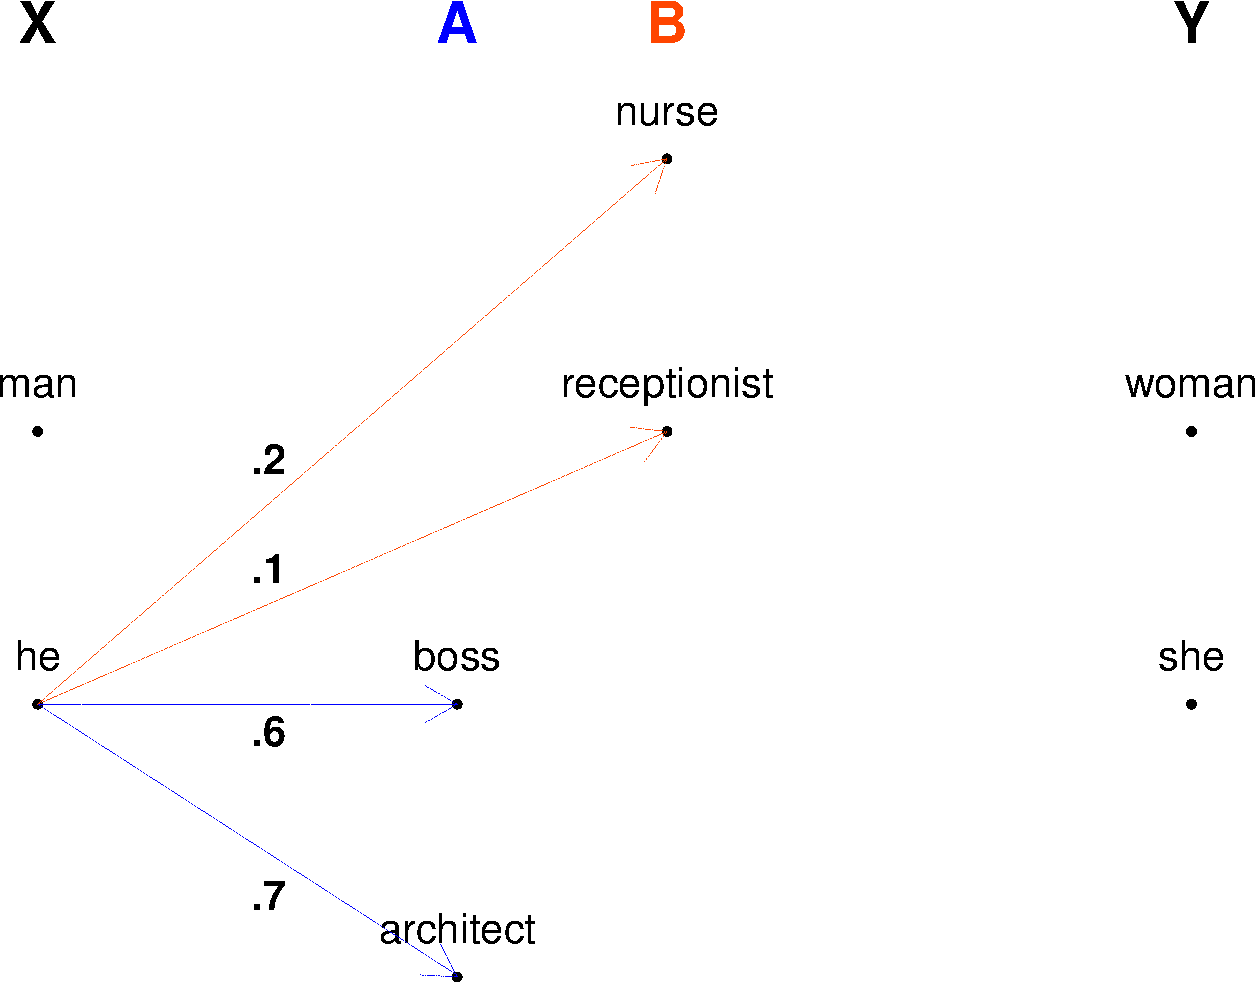
\includegraphics[width=1\linewidth]{_main_files/figure-latex/unnamed-chunk-2-1} \end{center}
\normalsize

The first impression is that while there is a shift for associated words towards smaller cosine distances as compared to the neutral words, slightly surprisingly a slightly weaker shift in the same direction is visible for attributes associated with different stereotypes. Moreover, the empirical distributions overlap to a large extent and the means grouped by connection type do not seem too far from each other. In fact, as there is a lot of variety in the cosine distances (as we will soon see), we need to gauge the uncertainty involved, and to look more carefully at individual protected words to get a better idea of how the cosine distance distribution changes for different attribute groups and different protected classes. Now, let's add the human attributes to the picture:

\vspace{1mm}
\footnotesize

\begin{center}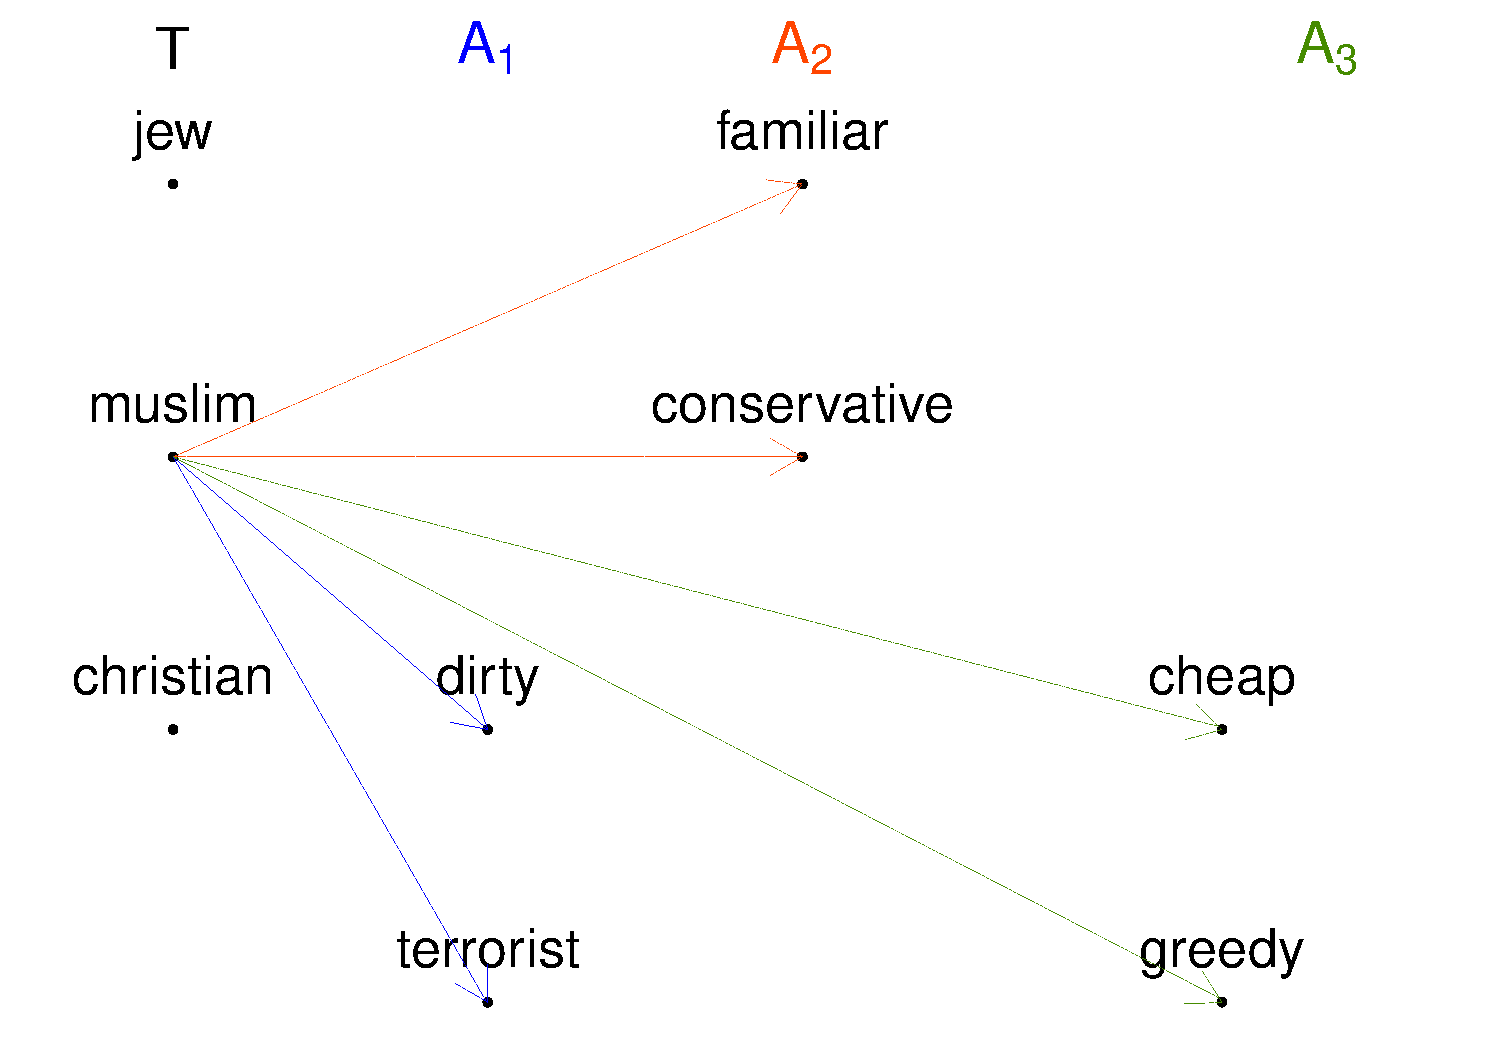
\includegraphics[width=1\linewidth]{_main_files/figure-latex/unnamed-chunk-3-1} \end{center}
\normalsize

\noindent Notice that the distribution for \texttt{human} (even though we did our best not to include in it any stereotype-related atributes) is left-skewed, with much overlap with \texttt{associated} and \texttt{different}, which illustrates the need to take being associated with humans as an important predictor.

Our focus lies in \texttt{connection} as a predictor. Morever, later on we'll be interested in looking at the protected words separately, and at protected words split by connection. For technical reasons it is useful to represent these factors as integer vectors.

\vspace{1mm}
\footnotesize

\begin{Shaded}
\begin{Highlighting}[]
\NormalTok{religion}\SpecialCharTok{$}\NormalTok{con }\OtherTok{\textless{}{-}} \FunctionTok{as.integer}\NormalTok{(religion}\SpecialCharTok{$}\NormalTok{connection)}
\end{Highlighting}
\end{Shaded}

\begin{verbatim}
## Warning: NAs introduced by coercion
\end{verbatim}

\begin{Shaded}
\begin{Highlighting}[]
\NormalTok{religion}\SpecialCharTok{$}\NormalTok{pw }\OtherTok{\textless{}{-}} \FunctionTok{as.integer}\NormalTok{(religion}\SpecialCharTok{$}\NormalTok{protectedWord)}
\end{Highlighting}
\end{Shaded}

\begin{verbatim}
## Warning: NAs introduced by coercion
\end{verbatim}

\begin{Shaded}
\begin{Highlighting}[]
\NormalTok{religion}\SpecialCharTok{$}\NormalTok{pwFactor }\OtherTok{\textless{}{-}} \FunctionTok{factor}\NormalTok{(}\FunctionTok{paste0}\NormalTok{(religion}\SpecialCharTok{$}\NormalTok{protectedWord, religion}\SpecialCharTok{$}\NormalTok{connection))}
\NormalTok{religion}\SpecialCharTok{$}\NormalTok{pwIndex }\OtherTok{\textless{}{-}} \FunctionTok{as.integer}\NormalTok{(religion}\SpecialCharTok{$}\NormalTok{pwFactor)}
\end{Highlighting}
\end{Shaded}

\normalsize

A short script, \texttt{cleanDataset} to make this faster, so equivalently:

\vspace{1mm}
\footnotesize

\begin{Shaded}
\begin{Highlighting}[]
\FunctionTok{source}\NormalTok{(}\StringTok{"../functions/cleanDataset.R"}\NormalTok{)}
\NormalTok{religion }\OtherTok{\textless{}{-}} \FunctionTok{read.csv}\NormalTok{(}\StringTok{"../datasets/religionReddit.csv"}\NormalTok{)[}\SpecialCharTok{{-}}\DecValTok{1}\NormalTok{]}
\NormalTok{religion }\OtherTok{\textless{}{-}} \FunctionTok{cleanDataset}\NormalTok{(religion,}\FunctionTok{c}\NormalTok{(}\StringTok{"christian"}\NormalTok{,}\StringTok{"human"}\NormalTok{,}\StringTok{"jewish"}\NormalTok{,}\StringTok{"muslim"}\NormalTok{,}\StringTok{"neutral"}\NormalTok{))}
\end{Highlighting}
\end{Shaded}

\begin{verbatim}
## Warning in cleanDataset(religion, c("christian", "human", "jewish", "muslim", :
## NAs introduced by coercion

## Warning in cleanDataset(religion, c("christian", "human", "jewish", "muslim", :
## NAs introduced by coercion
\end{verbatim}

\normalsize

\hypertarget{looking-at-the-islam-related-words}{%
\section{Looking at the islam-related words}\label{looking-at-the-islam-related-words}}

For now, let's focus on five protected words related to islam (``imam,'' ``islam,'' ``mosque,'' ``muslim,'' and ``quran''). The word list associates with islam four stereotypical attributes (``violent,'' ``terrorist,'' ``uneducated'' and ``dirty''). First, we select and plot the empirical distributions for these protected words.

\vspace{1mm}
\footnotesize

\begin{center}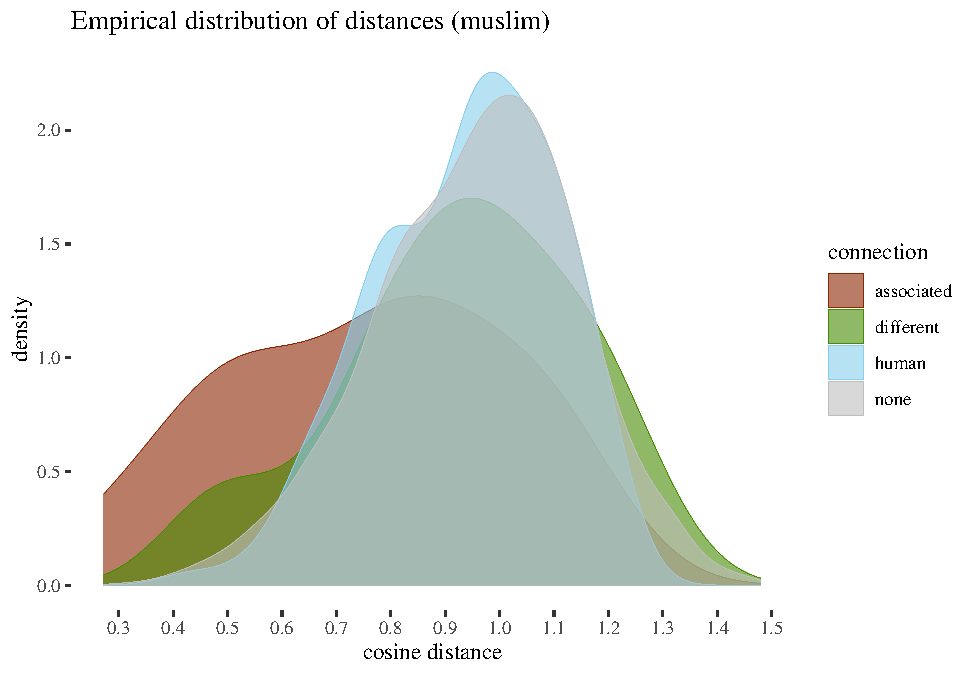
\includegraphics[width=1\linewidth]{_main_files/figure-latex/unnamed-chunk-6-1} \end{center}
\normalsize

\noindent Once we focus on words related to islam, the associated bias seems to be stronger than in the whole dataset. This is a step towards illustrating that the distribution of bias is uneven.

Now, say we want to look at a single protected word. Since the dataset also contains comparison multiple control neutral and human attributes, we randomly select only 5 from \texttt{none} and 5 from \texttt{human} control groups of those for the visualisation purposes.

\vspace{1mm}
\footnotesize

\begin{center}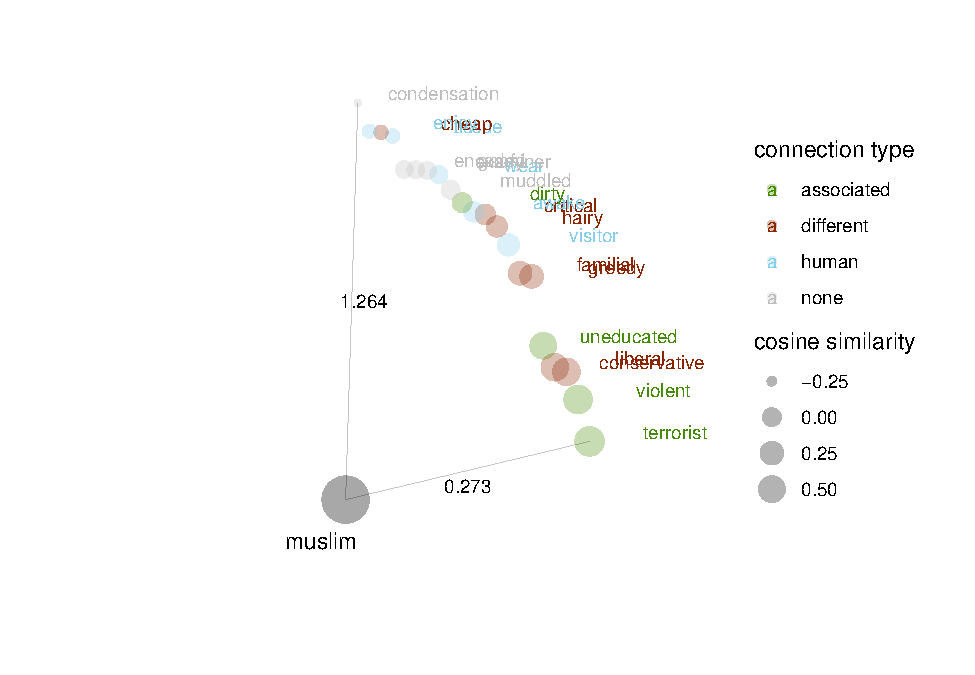
\includegraphics[width=1\linewidth]{_main_files/figure-latex/tableMuslimActive-1} \end{center}
\normalsize

Note that the distance between the grey point and the other points is proportional to cosine distance, the non-grey point size is proportional to cosine similarity to the protected word, and color groups by the connection type. So for \texttt{muslim} it seems that the stereotypes coming from the word list are fairly well visible. To give you some taste of how uneven the dataset is, compare this to what happens with \texttt{priest}.

\vspace{1mm}
\footnotesize

\begin{center}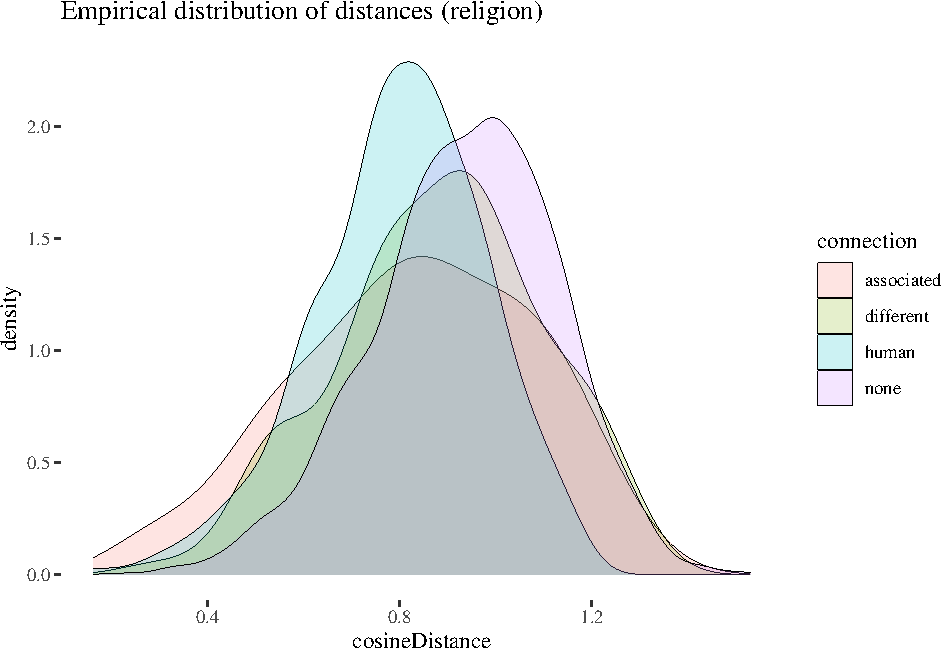
\includegraphics[width=1\linewidth]{_main_files/figure-latex/unnamed-chunk-7-1} \end{center}
\normalsize

\noindent Here you can see that some human attributes are closer than stereotype attributes, and that there is no clear reason to claim that \texttt{associated} attributes are closer than \texttt{different} or \texttt{human} attributes. This, again, illustrates the need of case-by-case analysis with control groups.

The general idea now is that the word lists provided in different pieces of research are just samples of attributes associates with various stereotypes and should be treated as such: the uncertainty involved and the sample sizes should have clear impact on our estimates.

\hypertarget{bayesian-model-structure-and-assumptions}{%
\section{Bayesian model structure and assumptions}\label{bayesian-model-structure-and-assumptions}}

We will now think of cosine distance as the output variable, and
will build a few Bayesian models to compare. First, we just build a baseline model which estimates cosine distance to the attributes separately for each protected word. The underlying idea is that different protected words might in general have different relations to all the attributes and these relations should be our point of departure.\footnote{The construction of the Bayesian models and code for visualisations is due to Rafal Urbaniak.}

Here is the intuition behind the mathematical Bayesian model involved. Our outcome variable is \texttt{cosine\ difference}, which we take to me normally distributed around the predicted mean for a given protected word (that is, we assume the residuals are normally distributed). The simplest model specification is:

\begin{align}
cosineDistance_i  & \sim dnorm(\mu_i, \sigma) \\
\mu_i & = m_{pw} \\
m_{pw} & ~ dnorm(1,.5) \\
\sigma &\sim  dcauchy(0,1)
\end{align}

That is, we assume the estimated means might be different for diferent protected words and our prior for the mean and the overal standard deviation are normal with mean 1 and sd=.5 and half-cauchy with parameters \texttt{0,1}. Further on we'll also estimate additional impact the connection type may have. For this impact we take a slightly skeptical prior centered around 0 distributed normally with sd = 1. These are fairly weak and slightly skeptical regularizing priors, which can be illustrated as follows:

\vspace{2mm}

\begin{center}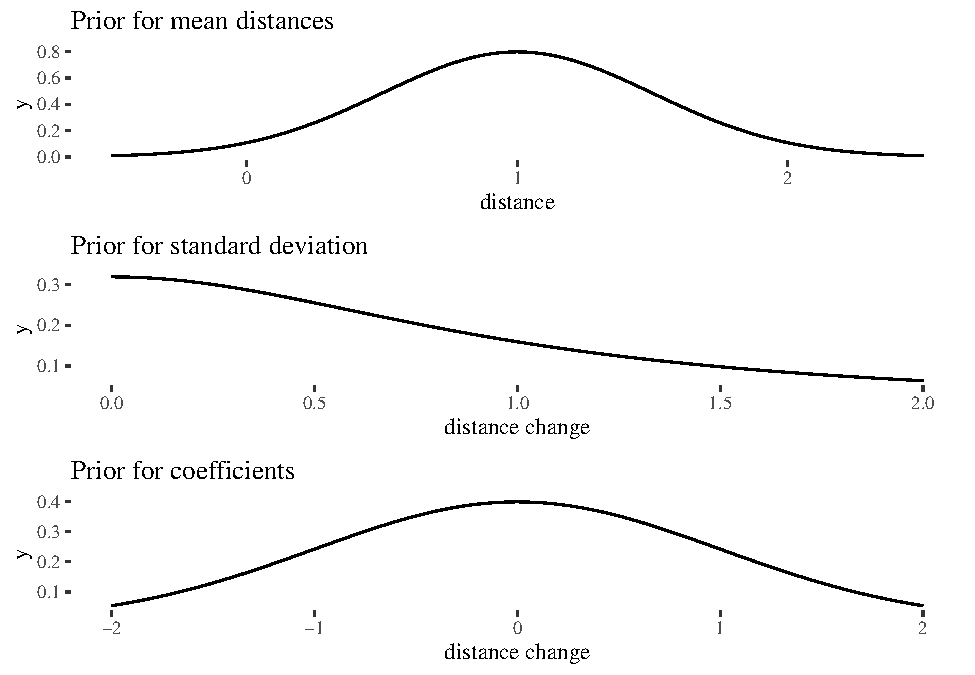
\includegraphics[width=1\linewidth]{_main_files/figure-latex/priorsVis-1} \end{center}

\hypertarget{choosing-predictors}{%
\section{Choosing predictors}\label{choosing-predictors}}

Now we can define and compile the baseline model. Its parameters will have a posterior distribution obtained using either Hamiltionian Monte Carlo methods (STAN) available through the \texttt{rethinking} package.

\vspace{1mm}
\footnotesize

\begin{Shaded}
\begin{Highlighting}[]
\FunctionTok{library}\NormalTok{(rethinking)}
\FunctionTok{options}\NormalTok{(}\AttributeTok{buildtools.check =} \ControlFlowTok{function}\NormalTok{(action) }\ConstantTok{TRUE}\NormalTok{ )}
\NormalTok{religionBaseline }\OtherTok{\textless{}{-}} \FunctionTok{ulam}\NormalTok{(}
  \FunctionTok{alist}\NormalTok{(}
\NormalTok{    cosineDistance }\SpecialCharTok{\textasciitilde{}} \FunctionTok{dnorm}\NormalTok{(mu,sigma),}
\NormalTok{    mu }\OtherTok{\textless{}{-}}\NormalTok{ m[pw],}
\NormalTok{    m[pw] }\SpecialCharTok{\textasciitilde{}} \FunctionTok{dnorm}\NormalTok{(}\DecValTok{1}\NormalTok{,.}\DecValTok{5}\NormalTok{),}
\NormalTok{    sigma }\SpecialCharTok{\textasciitilde{}} \FunctionTok{dcauchy}\NormalTok{(}\DecValTok{0}\NormalTok{,}\DecValTok{1}\NormalTok{)}
\NormalTok{  ),}
  \AttributeTok{data =}\NormalTok{ religion,}
  \AttributeTok{chains=}\DecValTok{2}\NormalTok{ , }\AttributeTok{iter=}\DecValTok{4000}\NormalTok{ , }\AttributeTok{warmup=}\DecValTok{1000}\NormalTok{,}
  \AttributeTok{start=} \FunctionTok{list}\NormalTok{(}\AttributeTok{mu =} \DecValTok{1}\NormalTok{, }\AttributeTok{co =} \DecValTok{0}\NormalTok{, }\AttributeTok{sigma=}\NormalTok{ .}\DecValTok{3}\NormalTok{),}
  \AttributeTok{log\_lik =} \ConstantTok{TRUE}\NormalTok{, }\AttributeTok{cores=}\DecValTok{4}
\NormalTok{)}
\CommentTok{\#saving}
\CommentTok{\#saveRDS(religionBaseline, }
\CommentTok{\#file = "cosineAnalysis/models/religionBaseline.rds")}
\end{Highlighting}
\end{Shaded}

\normalsize

The only reason we need it is the evaluation of connection as a predictor. Does including it in o the model improve the situation? To investigate this, let's now build a model according to the following specification:

\begin{align}
cosineDistance_i  & \sim dnorm(\mu_i, \sigma) \\
\mu_i & = m_{pw} + co_{con}\\
m_{pw} & ~ dnorm(1,.5) \\
co_{con} & ~ dnorm(0,1) \\
\sigma &\sim  dcauchy(0,1)
\end{align}

\noindent The idea now is that each connection type comes with its own coefficient \(co\) that has impact on mean distances for protected words taken separately.

\vspace{1mm}
\footnotesize

\begin{Shaded}
\begin{Highlighting}[]
\FunctionTok{library}\NormalTok{(rethinking)}
\FunctionTok{options}\NormalTok{(}\AttributeTok{buildtools.check =} \ControlFlowTok{function}\NormalTok{(action) }\ConstantTok{TRUE}\NormalTok{ )}
\NormalTok{religionCoefs }\OtherTok{\textless{}{-}} \FunctionTok{ulam}\NormalTok{(}
  \FunctionTok{alist}\NormalTok{(}
\NormalTok{    cosineDistance }\SpecialCharTok{\textasciitilde{}} \FunctionTok{dnorm}\NormalTok{(mu,sigma),}
\NormalTok{    mu }\OtherTok{\textless{}{-}}\NormalTok{ m[pw] }\SpecialCharTok{+}\NormalTok{ co[con],}
\NormalTok{    m[pw] }\SpecialCharTok{\textasciitilde{}} \FunctionTok{dnorm}\NormalTok{(}\DecValTok{1}\NormalTok{,.}\DecValTok{5}\NormalTok{),}
\NormalTok{    co[con] }\SpecialCharTok{\textasciitilde{}}\FunctionTok{dnorm}\NormalTok{(}\DecValTok{0}\NormalTok{,.}\DecValTok{5}\NormalTok{),}
\NormalTok{    sigma }\SpecialCharTok{\textasciitilde{}} \FunctionTok{dcauchy}\NormalTok{(}\DecValTok{0}\NormalTok{,}\DecValTok{1}\NormalTok{)}
\NormalTok{  ),}
  \AttributeTok{data =}\NormalTok{ religion,}
  \AttributeTok{chains=}\DecValTok{2}\NormalTok{ , }\AttributeTok{iter=}\DecValTok{8000}\NormalTok{ , }\AttributeTok{warmup=}\DecValTok{1000}\NormalTok{, }
  \AttributeTok{log\_lik =} \ConstantTok{TRUE}
\NormalTok{)}
\end{Highlighting}
\end{Shaded}

\normalsize

\noindent First, let's see if this model is really better in terms of the Widely Acceptable Information Criterion (WAIC):

\vspace{1mm}
\footnotesize

\begin{verbatim}
##                   WAIC SE dWAIC dSE pWAIC weight
## religionCoefs    -2328 93     0  NA    20      1
## religionBaseline -2283 95    45  17    16      0
\end{verbatim}

\normalsize

Clearly, it should be given weight 1 as compared to the baseline model. So far, we've learned that the connection type actually has predictive value. Let's take a look at the coefficient estimates:

\vspace{1mm}
\footnotesize

\begin{verbatim}
##              mean        sd       5.5%      94.5%    n_eff    Rhat4
## co[1] -0.14956420 0.1151675 -0.3261650 0.03741930 294.2033 1.001449
## co[2] -0.09880543 0.1145024 -0.2736985 0.08813271 291.5044 1.001564
## co[3] -0.07282752 0.1133894 -0.2447778 0.11158986 287.7820 1.001627
## co[4] -0.03103179 0.1131420 -0.2034442 0.15268770 286.8283 1.001606
\end{verbatim}

\normalsize

\hypertarget{dataset-level-coefficients}{%
\section{\texorpdfstring{Dataset-level coefficients \label{sec:datasetsLevelCoeffs}}{Dataset-level coefficients }}\label{dataset-level-coefficients}}

\noindent Let's plot them together with their highest posterior density invervals, for the three topic groups.

\begin{center}
\begin{figure}[!htb]\centering
   \begin{minipage}{0.55\textwidth}
  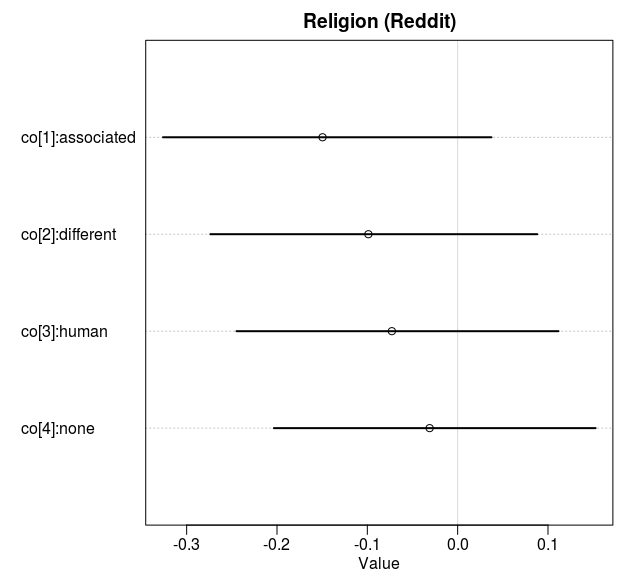
\includegraphics[width=7cm]{../images/religionCoeffs.jpeg}
   \end{minipage}
   \begin {minipage}{0.43\textwidth}
    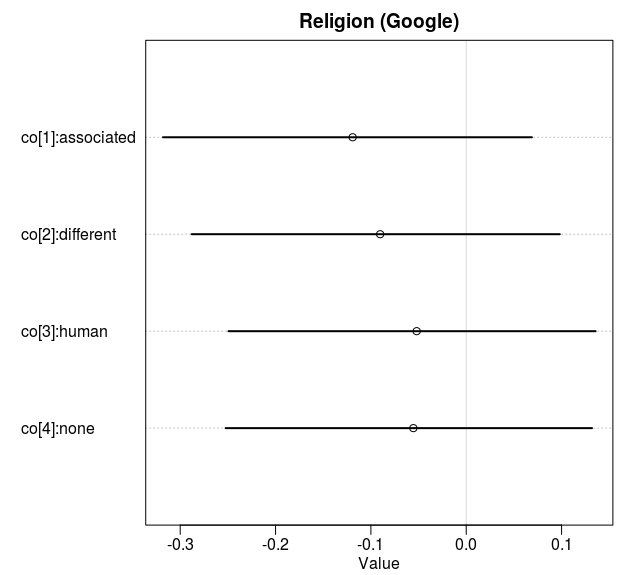
\includegraphics[width=7cm]{../images/religionGoogleCoeffs.jpeg}
   \end{minipage}
   
   
  \begin{minipage}{0.55\textwidth}
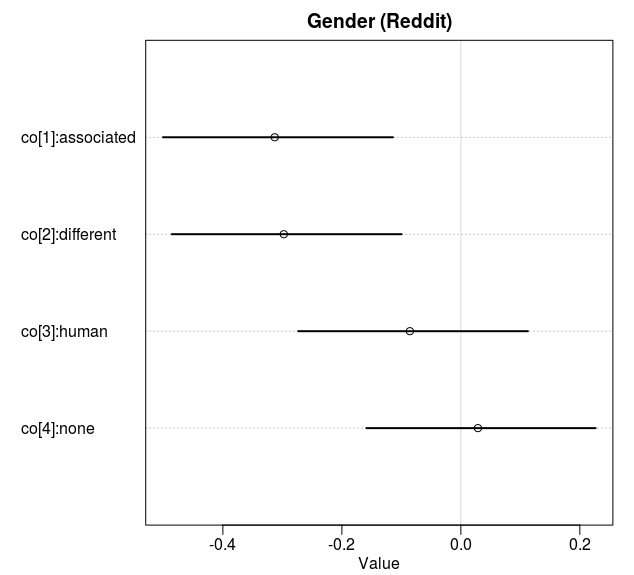
\includegraphics[width=7cm]{../images/genderCoeffs.jpeg}
\end{minipage}
   \begin {minipage}{0.43\textwidth}
    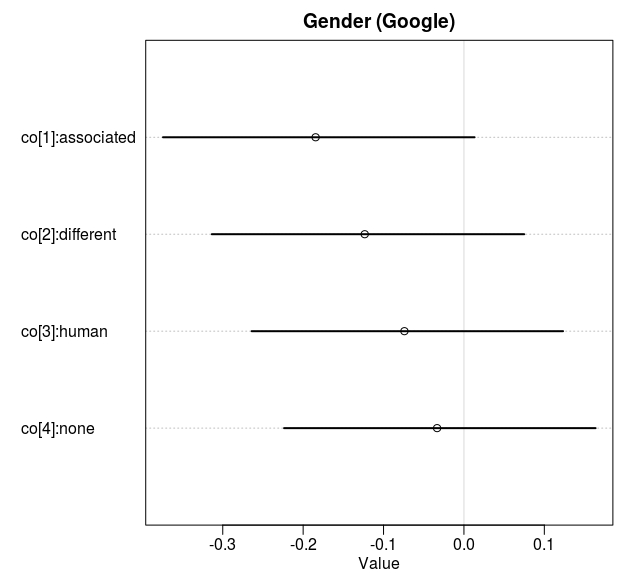
\includegraphics[width=7cm]{../images/genderGoogleCoeffs.jpeg}
   \end{minipage}
   
   
   
   
  \begin{minipage}{0.55\textwidth}
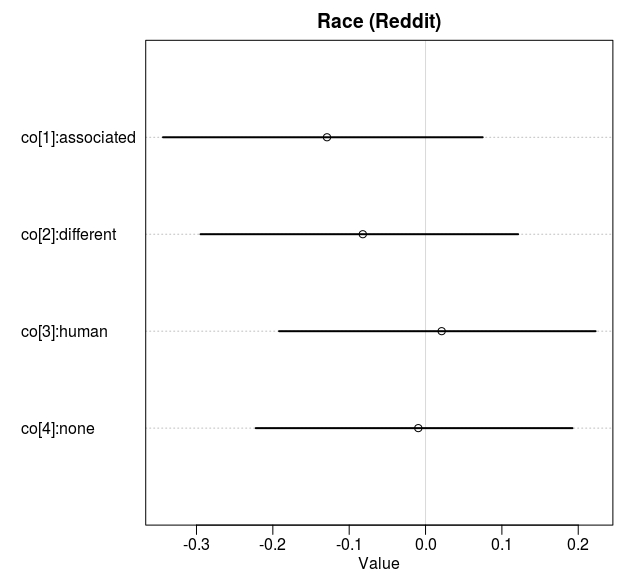
\includegraphics[width=7cm]{../images/raceCoeffs.jpeg}
\end{minipage}
   \begin {minipage}{0.43\textwidth}
    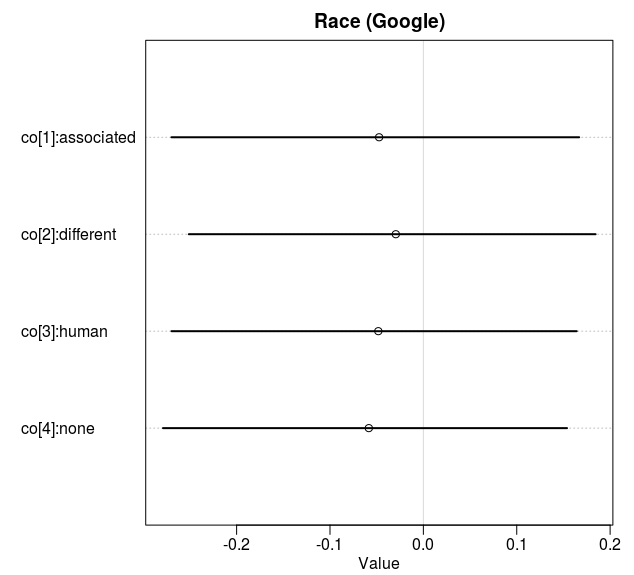
\includegraphics[width=7cm]{../images/raceGoogleCoeffs.jpeg}
   \end{minipage}
\end{figure}


\end{center}

\noindent What should strike us is that while the mean estimates of the coefficients indeed do differ a bit, usually the highest posterior density invervals all include zero, and so we do not have strong reasons to say that, say, as far as the whole religion dataset is involved, being associated indeed is connected with lower cosine distance. A second striking observation is that the estimated impact for associated stereotypes is quite often not too different from the estimated impact of attributes associated with different stereotypes, and both are sometimes not too far from the estimated impact for simply human attributes. In general, once the uncertainty involved is taken seriously by using control groups and statistical uncertainty estimation that does not dispose of pointwise data, the picture which focuses only on differences between means of means is too simplistic.

But this doesn't mean important differences for some protected words are not there. For one thing, if you start with a word list that is very uneven, the actually not so bad status of some of the protected words might mask a pretty bad situation in which some other protected words are. For comparison, let's see what a model focused on words related to islam tells us.

\vspace{1mm}
\footnotesize

\begin{Shaded}
\begin{Highlighting}[]
\CommentTok{\#this is how we build the model}
\NormalTok{religion }\OtherTok{\textless{}{-}} \FunctionTok{read.csv}\NormalTok{(}\StringTok{"cosineAnalysis/datasets/religionReddit.csv"}\NormalTok{)[}\SpecialCharTok{{-}}\DecValTok{1}\NormalTok{]}
\FunctionTok{colnames}\NormalTok{(religion) }\OtherTok{\textless{}{-}} \FunctionTok{c}\NormalTok{(}\StringTok{"protectedWord"}\NormalTok{,}\StringTok{"wordToCompare"}\NormalTok{,}\StringTok{"wordClass"}\NormalTok{,}
                        \StringTok{"cosineDistance"}\NormalTok{,}\StringTok{"cosineSimilarity"}\NormalTok{,}\StringTok{"connection"}\NormalTok{)}
\FunctionTok{levels}\NormalTok{(religion}\SpecialCharTok{$}\NormalTok{wordClass) }\OtherTok{\textless{}{-}} \FunctionTok{c}\NormalTok{(}\StringTok{"christian"}\NormalTok{,}\StringTok{"human"}\NormalTok{,}\StringTok{"jewish"}\NormalTok{,}\StringTok{"muslim"}\NormalTok{,}\StringTok{"neutral"}\NormalTok{)}
\NormalTok{muslimWords }\OtherTok{\textless{}{-}} \FunctionTok{c}\NormalTok{(}\StringTok{"imam"}\NormalTok{,}\StringTok{"islam"}\NormalTok{,}\StringTok{"mosque"}\NormalTok{,}\StringTok{"muslim"}\NormalTok{,}\StringTok{"quran"}\NormalTok{)}
\NormalTok{muslim }\OtherTok{\textless{}{-}}\NormalTok{ religion }\SpecialCharTok{\%\textgreater{}\%} \FunctionTok{filter}\NormalTok{(protectedWord }\SpecialCharTok{\%in\%}\NormalTok{ muslimWords)}
\NormalTok{muslim}\SpecialCharTok{$}\NormalTok{protectedWord }\OtherTok{\textless{}{-}} \FunctionTok{droplevels}\NormalTok{(muslim}\SpecialCharTok{$}\NormalTok{protectedWord)}
\NormalTok{muslim}\SpecialCharTok{$}\NormalTok{pw }\OtherTok{\textless{}{-}} \FunctionTok{as.integer}\NormalTok{(muslim}\SpecialCharTok{$}\NormalTok{protectedWord)}
\NormalTok{muslim}\SpecialCharTok{$}\NormalTok{con }\OtherTok{\textless{}{-}} \FunctionTok{as.integer}\NormalTok{(muslim}\SpecialCharTok{$}\NormalTok{connection)}
\NormalTok{muslim}\SpecialCharTok{$}\NormalTok{pwFactor }\OtherTok{\textless{}{-}} \FunctionTok{factor}\NormalTok{(}\FunctionTok{paste0}\NormalTok{(muslim}\SpecialCharTok{$}\NormalTok{protectedWord, muslim}\SpecialCharTok{$}\NormalTok{connection))}
\NormalTok{muslim}\SpecialCharTok{$}\NormalTok{pwIndex }\OtherTok{\textless{}{-}} \FunctionTok{as.integer}\NormalTok{(muslim}\SpecialCharTok{$}\NormalTok{pwFactor)}

\NormalTok{islamCoefs }\OtherTok{\textless{}{-}} \FunctionTok{ulam}\NormalTok{(}
  \FunctionTok{alist}\NormalTok{(}
\NormalTok{    cosineDistance }\SpecialCharTok{\textasciitilde{}} \FunctionTok{dnorm}\NormalTok{(mu,sigma),}
\NormalTok{    mu }\OtherTok{\textless{}{-}}\NormalTok{ m[pw] }\SpecialCharTok{+}\NormalTok{ co[con],}
\NormalTok{    m[pw] }\SpecialCharTok{\textasciitilde{}} \FunctionTok{dnorm}\NormalTok{(}\DecValTok{1}\NormalTok{,.}\DecValTok{5}\NormalTok{),}
\NormalTok{    co[con] }\SpecialCharTok{\textasciitilde{}}\FunctionTok{dnorm}\NormalTok{(}\DecValTok{0}\NormalTok{,.}\DecValTok{5}\NormalTok{),}
\NormalTok{    sigma }\SpecialCharTok{\textasciitilde{}} \FunctionTok{dcauchy}\NormalTok{(}\DecValTok{0}\NormalTok{,}\DecValTok{1}\NormalTok{)}
\NormalTok{  ),}
  \AttributeTok{data =}\NormalTok{ muslim,}
  \AttributeTok{chains=}\DecValTok{2}\NormalTok{ , }\AttributeTok{iter=}\DecValTok{10000}\NormalTok{ , }\AttributeTok{warmup=}\DecValTok{1000}\NormalTok{, }\AttributeTok{cores =} \DecValTok{4}\NormalTok{,}
  \AttributeTok{log\_lik =} \ConstantTok{TRUE}
\NormalTok{)}
\end{Highlighting}
\end{Shaded}

\normalsize

Let's take a look at the coefficients:

\vspace{1mm}
\footnotesize

\begin{verbatim}
##                mean        sd       5.5%      94.5%    n_eff    Rhat4
## co[1] -0.1979930035 0.1708785 -0.4682696 0.07634977 1789.894 1.003445
## co[2] -0.0334215769 0.1687587 -0.3021954 0.23720938 1738.720 1.003575
## co[3] -0.0192492753 0.1675754 -0.2840596 0.24860974 1732.907 1.003755
## co[4] -0.0003911363 0.1670610 -0.2661047 0.26815172 1723.758 1.003837
\end{verbatim}

\normalsize

\begin{center}
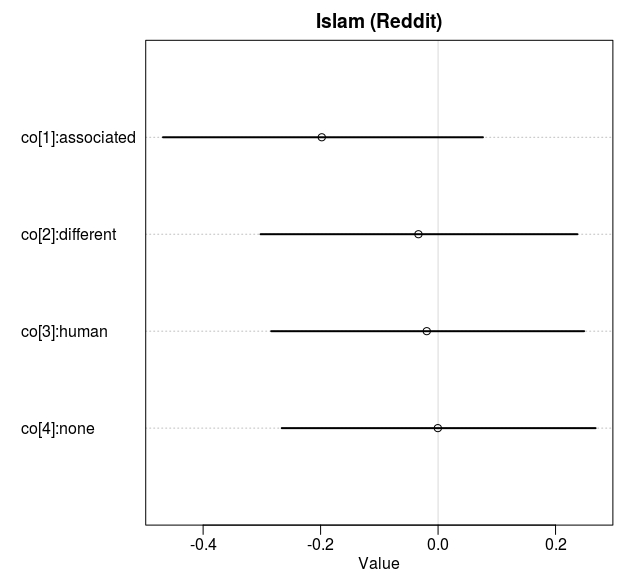
\includegraphics[width=8cm]{../images/islamCoeffs.jpeg}
\end{center}

\normalsize

While muslim words were unusual in the sense that the disparity between associated attributes and others is stronger, the evidence is still not conclusive. This is because the variation even within islam-related words is large enough (and sample sizes sufficiently small) for all the highest posterior density invervals to still include zeros.

So, it seems, taking a closer look does seem to make a difference. The question is, what happens if we do take a close look at the level of protected words?

\hypertarget{protected-word-level-analysis}{%
\chapter{Protected-word level analysis}\label{protected-word-level-analysis}}

\hypertarget{model-structure-and-assumptions}{%
\section{Model structure and assumptions}\label{model-structure-and-assumptions}}

Let's turn then to data analysis that takes a look at protected words separately. This time, for each combination of a protected word and a connection status we will have a separate mean cosine distance estimate, each coming with its own highest posterior density interval. This means we will use indices that are result from all such combinations (and then we will split them up in the model precis to build visualisation, feel free to look at the \texttt{visualiseStats.R} script for details).

\vspace{1mm}
\footnotesize

\begin{Shaded}
\begin{Highlighting}[]
\FunctionTok{options}\NormalTok{(}\AttributeTok{buildtools.check =} \ControlFlowTok{function}\NormalTok{(action) }\ConstantTok{TRUE}\NormalTok{ ) }\CommentTok{\#removes install pop{-}up request}
\NormalTok{religion}\SpecialCharTok{$}\NormalTok{pwFactor }\OtherTok{\textless{}{-}} \FunctionTok{factor}\NormalTok{(}\FunctionTok{paste0}\NormalTok{(religion}\SpecialCharTok{$}\NormalTok{protectedWord, }\StringTok{"{-}"}\NormalTok{, religion}\SpecialCharTok{$}\NormalTok{connection))}
\NormalTok{religion}\SpecialCharTok{$}\NormalTok{pwIndex }\OtherTok{\textless{}{-}} \FunctionTok{as.integer}\NormalTok{(religion}\SpecialCharTok{$}\NormalTok{pwFactor)}

\NormalTok{religionSeparate }\OtherTok{\textless{}{-}} \FunctionTok{ulam}\NormalTok{(}
  \FunctionTok{alist}\NormalTok{(}
\NormalTok{    cosineDistance }\SpecialCharTok{\textasciitilde{}} \FunctionTok{dnorm}\NormalTok{(mu,sigma),}
\NormalTok{    mu }\OtherTok{\textless{}{-}}\NormalTok{ c[pwIndex],}
\NormalTok{    c[pwIndex] }\SpecialCharTok{\textasciitilde{}} \FunctionTok{dnorm}\NormalTok{(}\DecValTok{1}\NormalTok{,.}\DecValTok{5}\NormalTok{),}
\NormalTok{    sigma }\SpecialCharTok{\textasciitilde{}} \FunctionTok{dcauchy}\NormalTok{(}\DecValTok{0}\NormalTok{,}\DecValTok{1}\NormalTok{)}
\NormalTok{  ),}
  \AttributeTok{data =}\NormalTok{ religion,}
  \AttributeTok{chains=}\DecValTok{2}\NormalTok{ , }\AttributeTok{iter=}\DecValTok{10000}\NormalTok{ , }\AttributeTok{warmup=}\DecValTok{1000}\NormalTok{,}
  \AttributeTok{start=}\FunctionTok{list}\NormalTok{(}\AttributeTok{no =} \DecValTok{1}\NormalTok{, }\AttributeTok{a =} \DecValTok{0}\NormalTok{, }\AttributeTok{d =} \DecValTok{0}\NormalTok{, }\AttributeTok{sigma=}\NormalTok{ .}\DecValTok{3}\NormalTok{), }\AttributeTok{log\_lik =}  \ConstantTok{TRUE}
\NormalTok{)}
\end{Highlighting}
\end{Shaded}

\normalsize

\noindent Let's see if the individualized model does better than the previous models in light of WAIC which does add penalty for the number of parameters.

\vspace{1mm}
\footnotesize

\begin{Shaded}
\begin{Highlighting}[]
\NormalTok{compareBaselineCoefsSeparate}\OtherTok{\textless{}{-}} \FunctionTok{readRDS}\NormalTok{(}\StringTok{"../datasets/compareBaselineCoefsSeparate.rds"}\NormalTok{)}
\NormalTok{compareBaselineCoefsSeparate}
\end{Highlighting}
\end{Shaded}

\begin{verbatim}
##                   WAIC SE dWAIC dSE pWAIC weight
## religionSeparate -2400 93     0  NA    60      1
## religionCoefs    -2328 93    72  29    20      0
## religionBaseline -2283 95   117  37    16      0
\end{verbatim}

\normalsize

\hypertarget{protected-classes-in-reddit-and-google-embeddings}{%
\section{Protected classes in Reddit and Google embeddings}\label{protected-classes-in-reddit-and-google-embeddings}}

It seems that we do want to prefer this model, despite its relative complication. Now, what does it tell us about the protected words? Let's visualise the predicted means together with 89\% highest posterior density intervals.

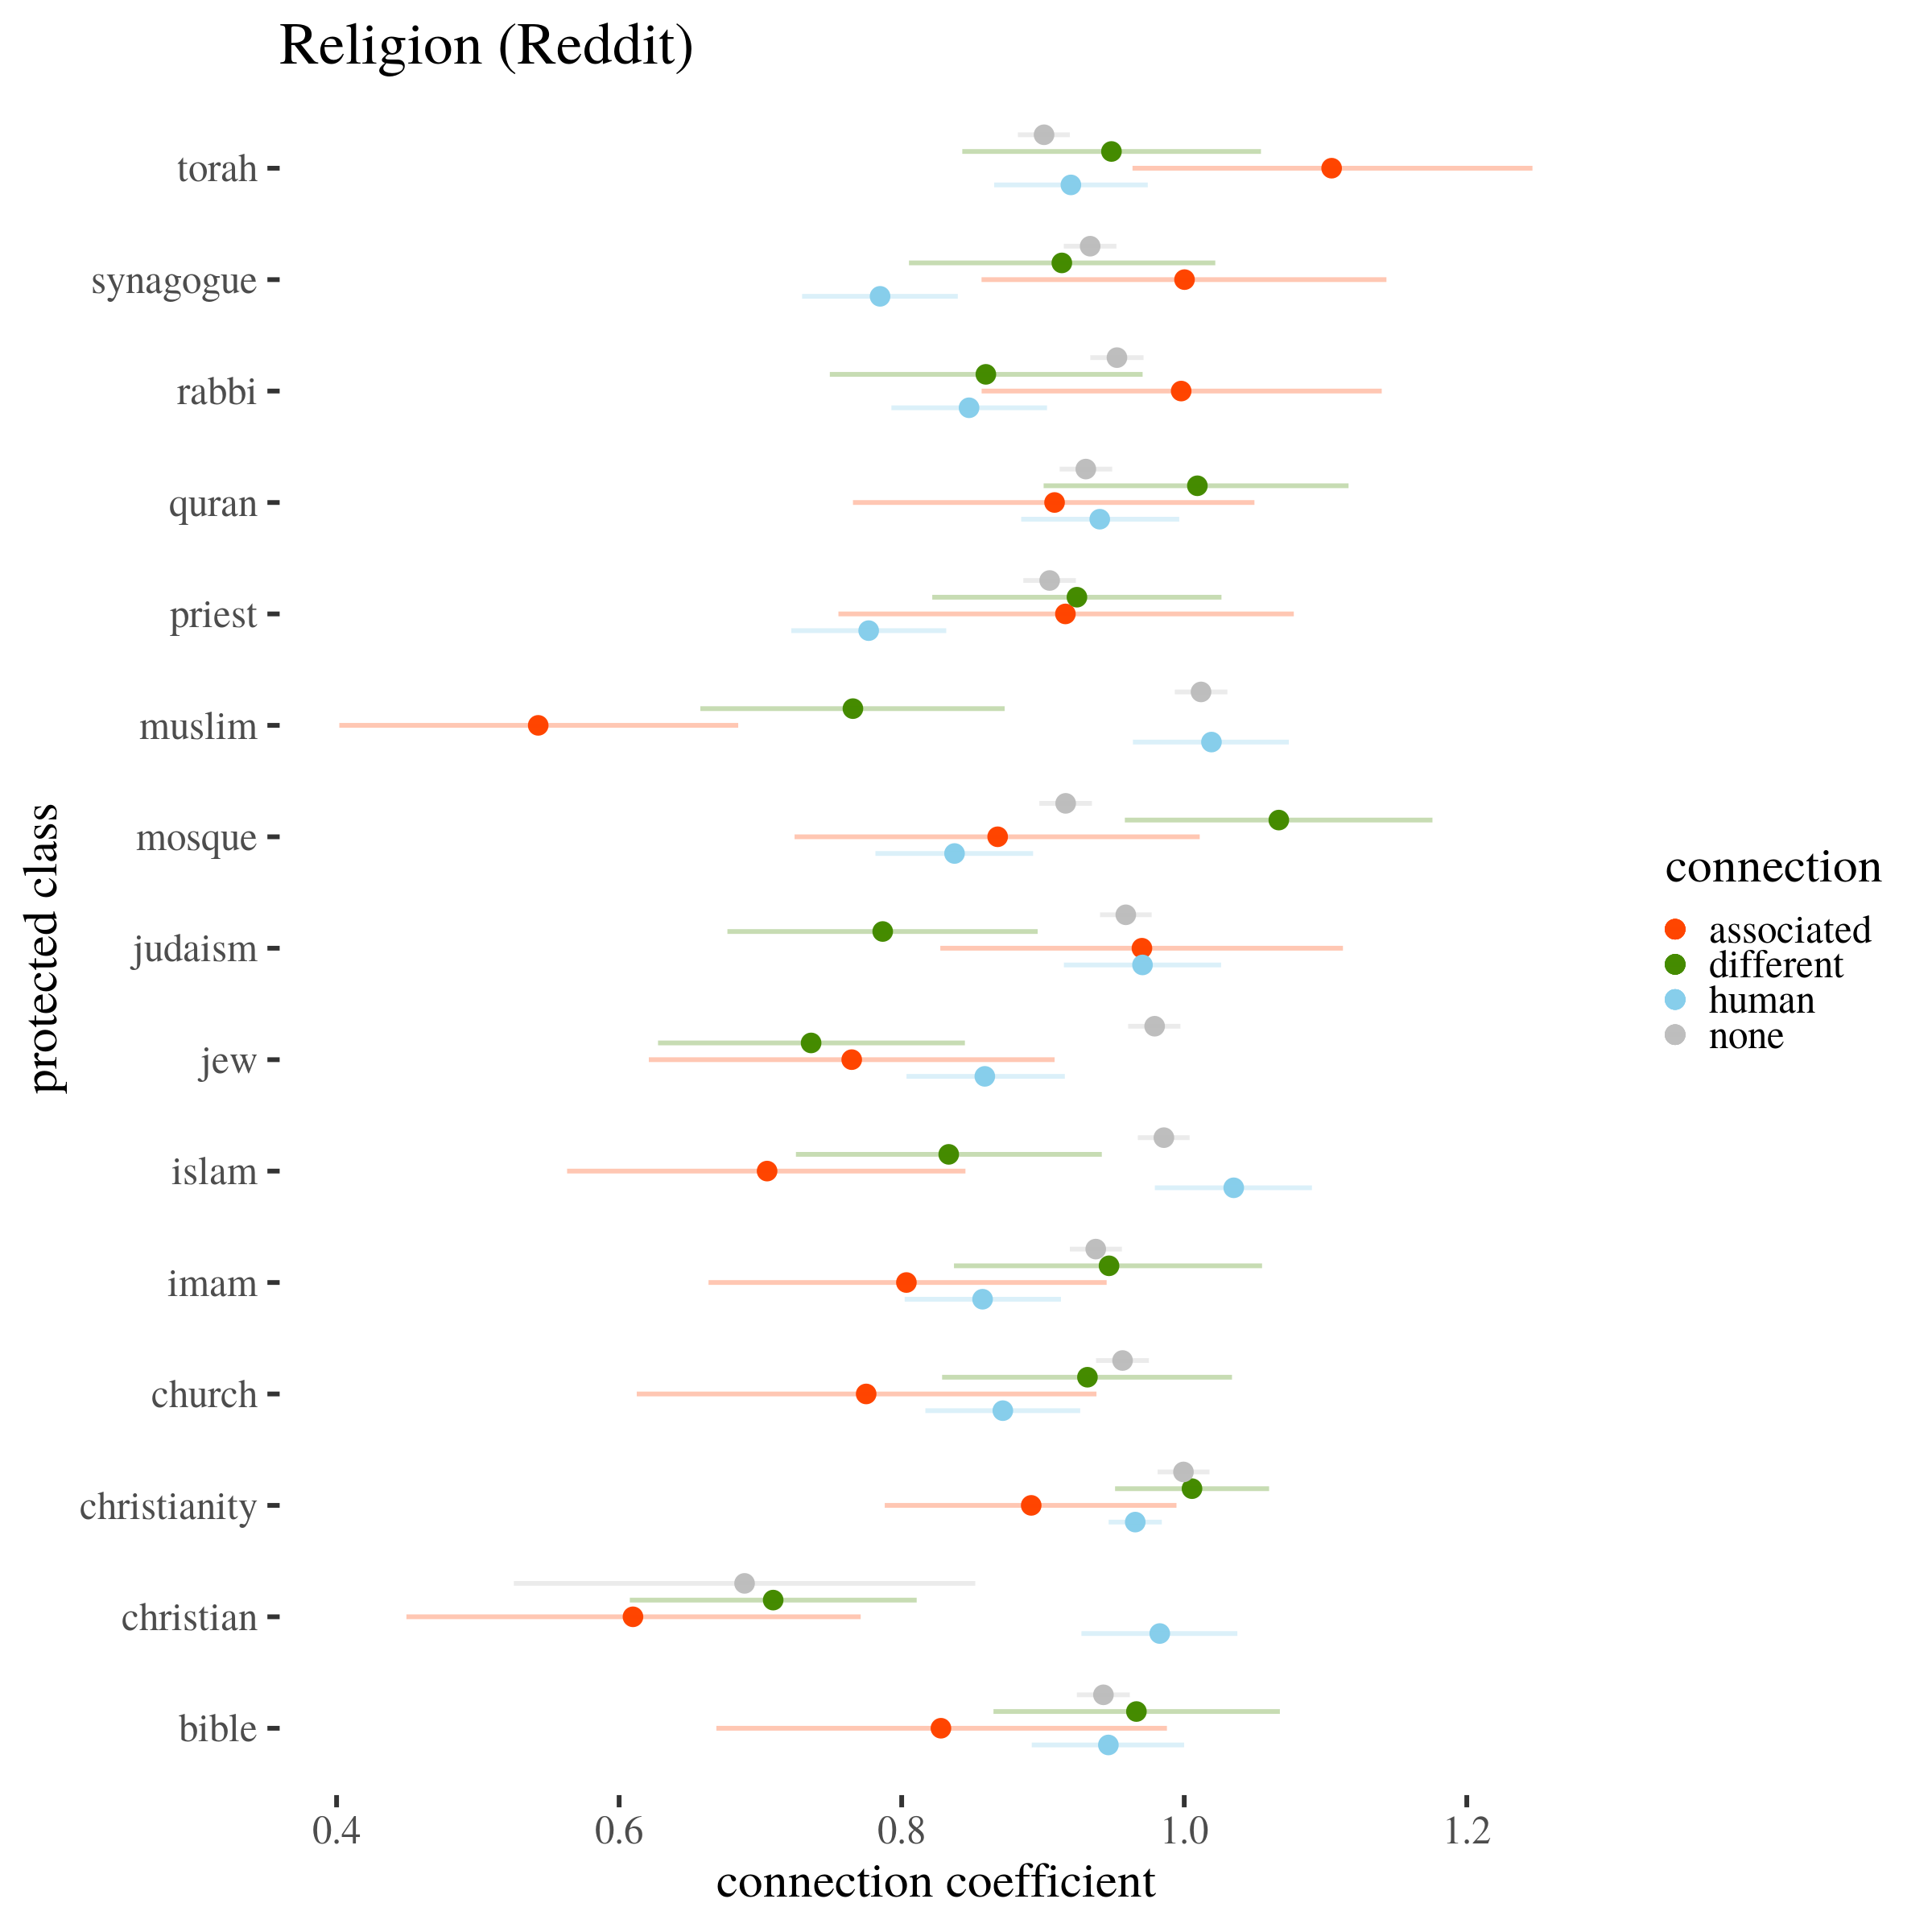
\includegraphics[width=14cm]{../images/visReligionReddit.png}

Before we move on, let's perform analogous analyses for the remaining types of supposed bias: gender and race (the model building is analogous).

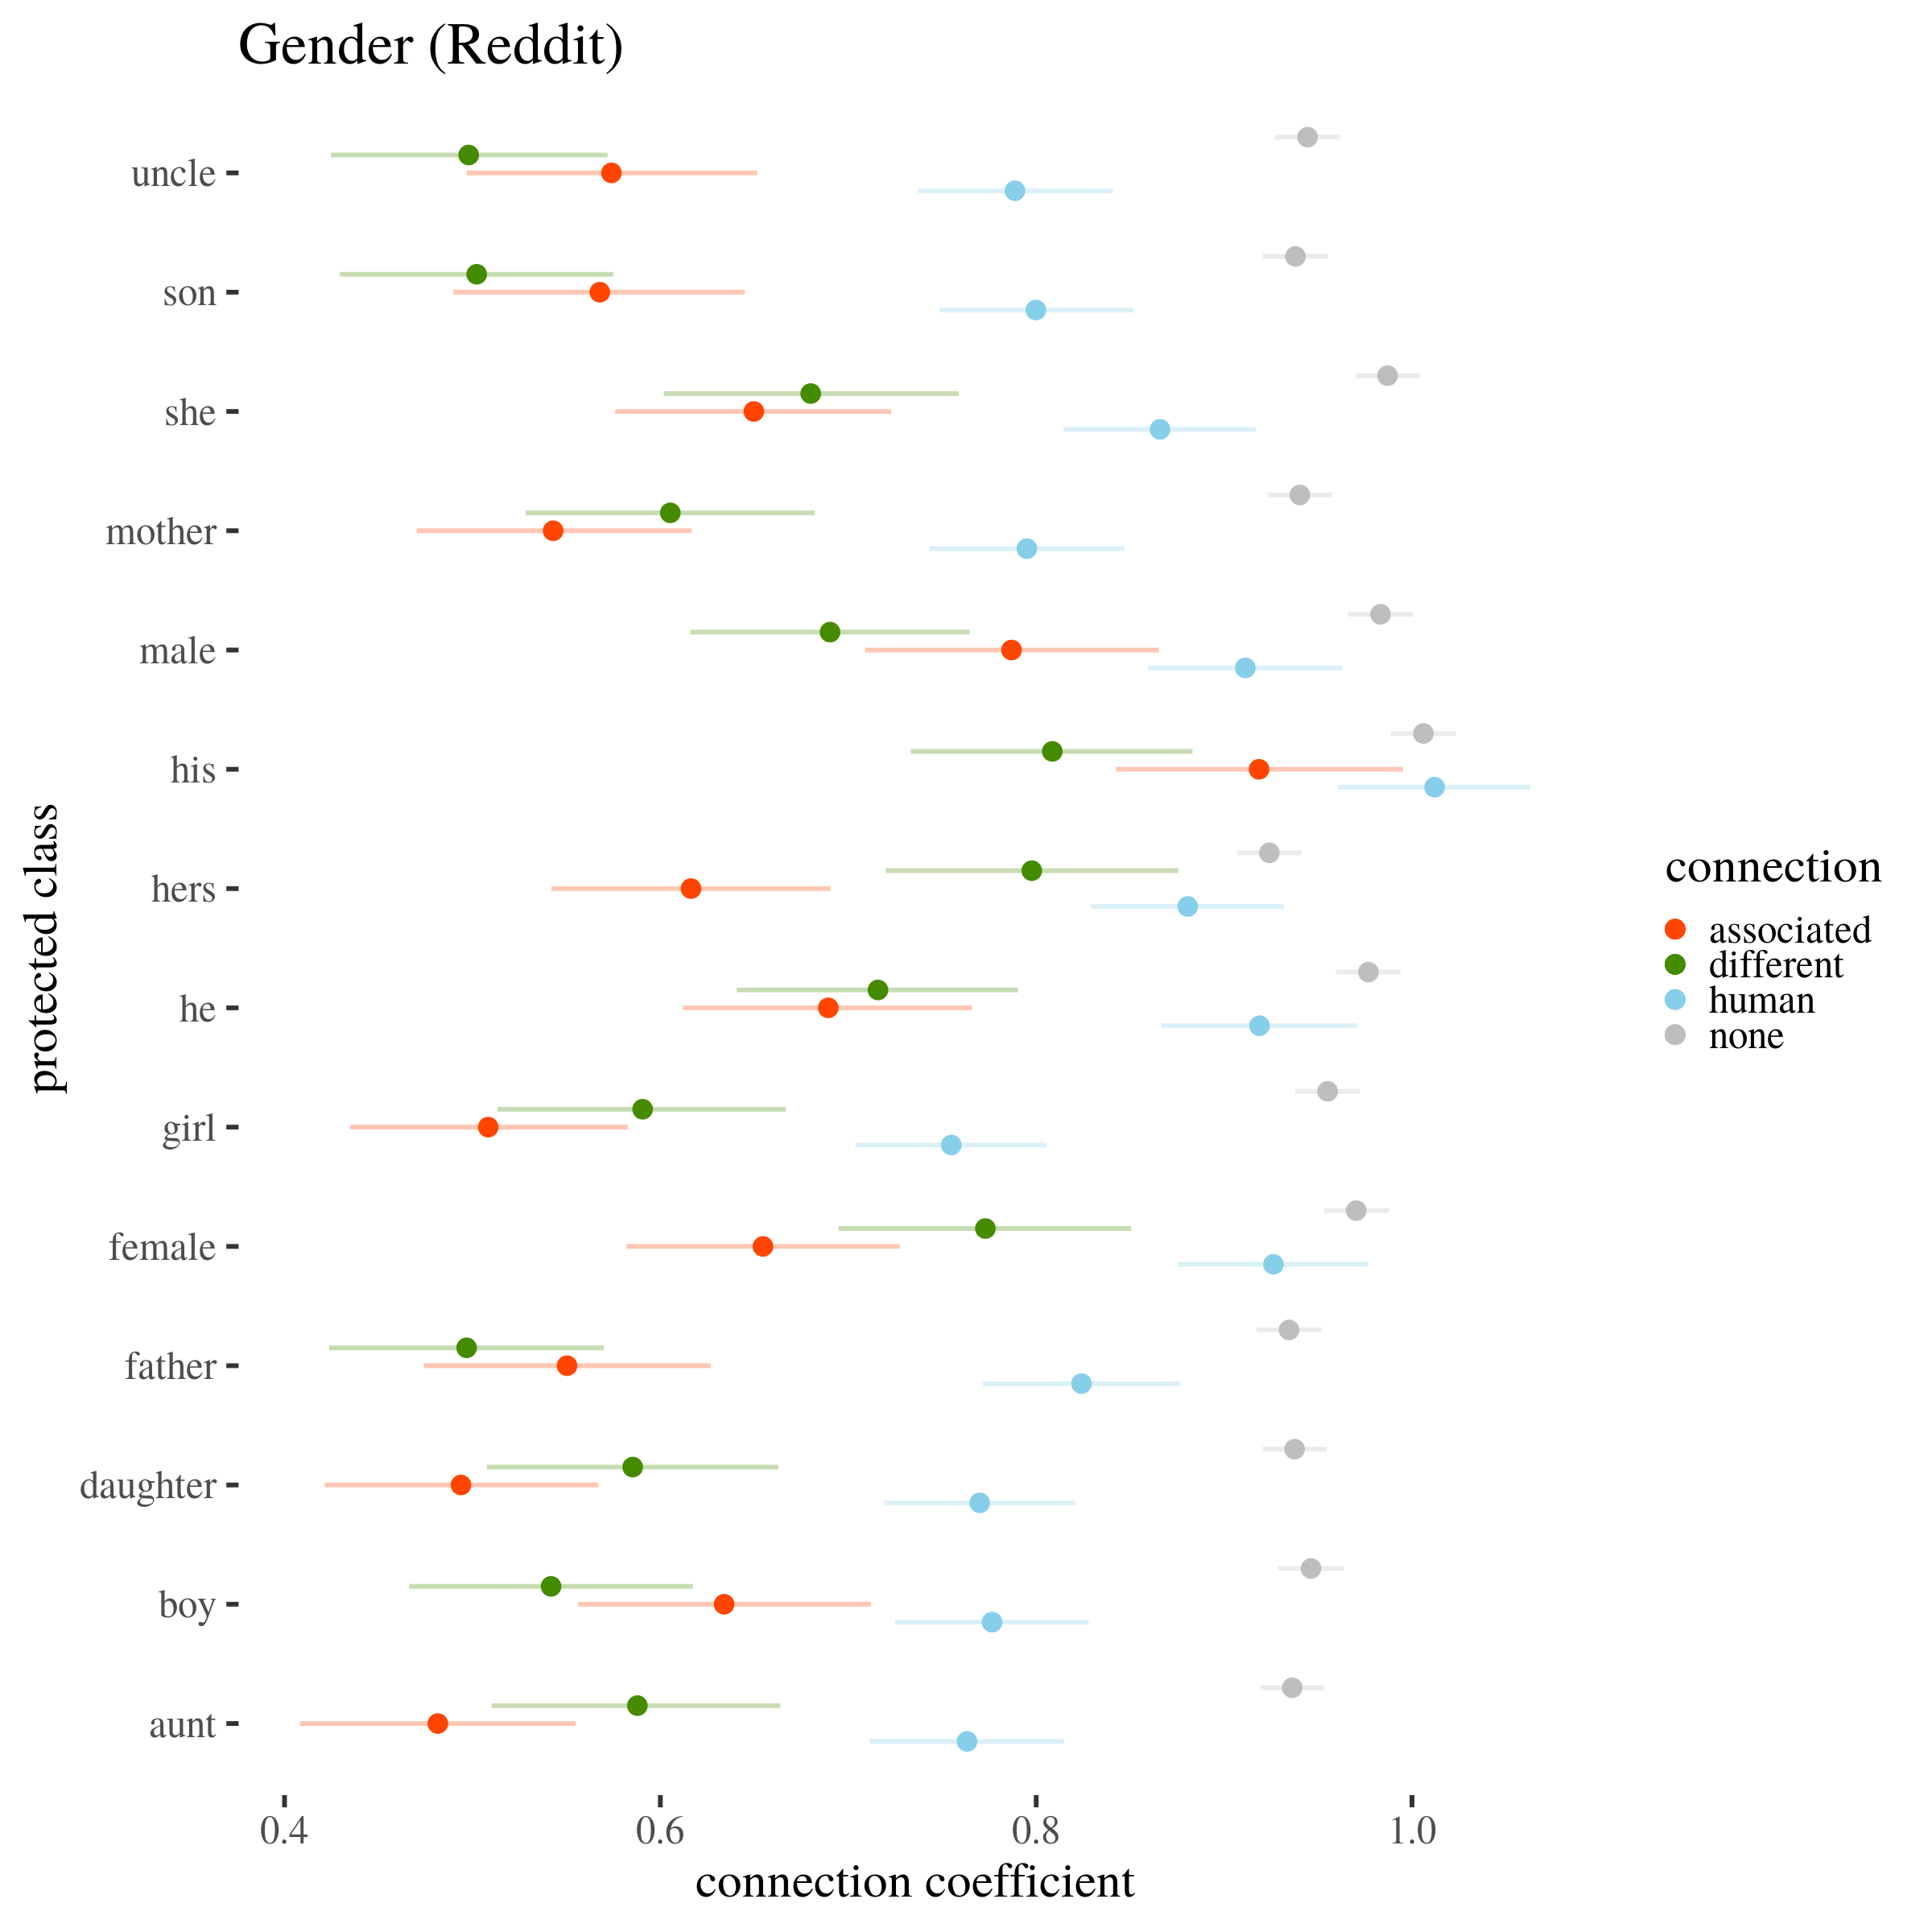
\includegraphics[width=14cm]{../images/visGenderReddit.png}

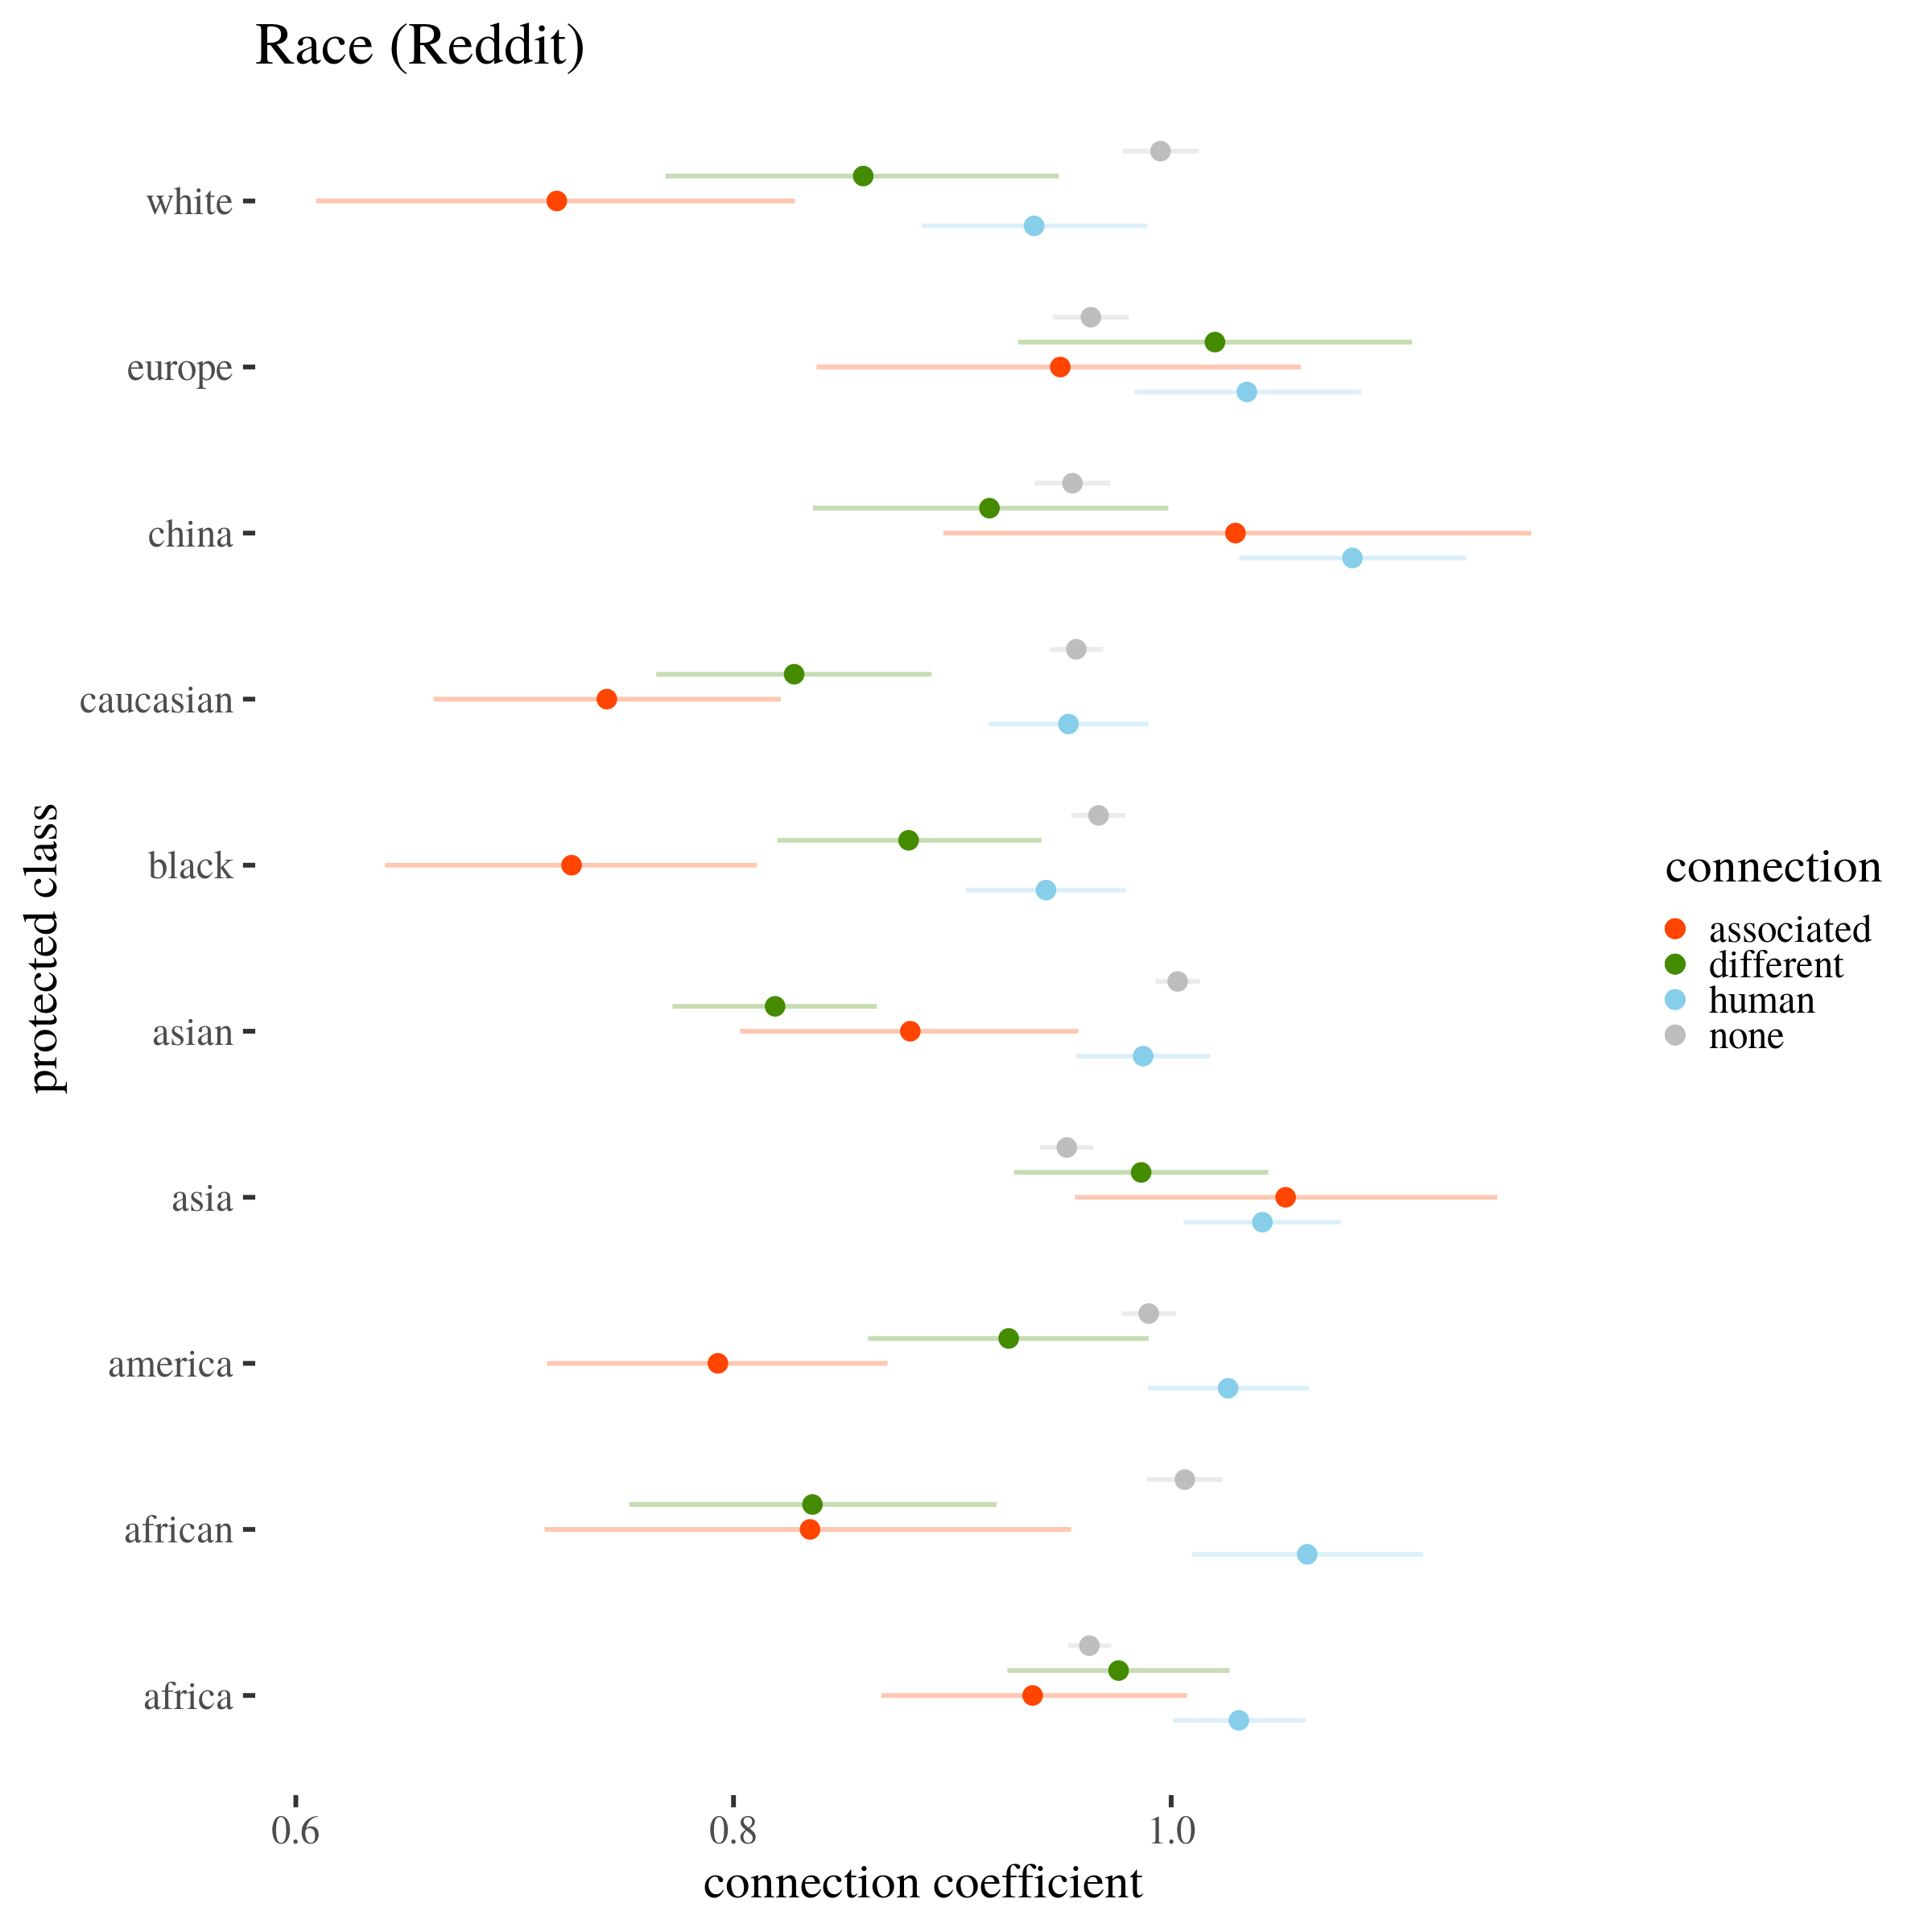
\includegraphics[width=14cm]{../images/visRaceReddit.png}

We first encountered the GoogleNews word embedding model in \protect\hyperlink{ref-Bolukbasi2016Man}{Bolukbasi, Chang, Zou, Saligrama, \& Kalai} (\protect\hyperlink{ref-Bolukbasi2016Man}{2016}). They use it for their calculations as written in \href{https://github.com/tolga-b/debiaswe}{Tolga Bolukbasi code}\footnote{\url{https://github.com/tolga-b/debiaswe}}. We decided to compare the results obtained with the use of Reddit L2 model and the ones that we got by GoogleNews model. The details of the model can be found here \href{https://code.google.com/archive/p/word2vec/}{Google News model}. One of the main differences between the models is that Reddit word embeggings have 50 dimensions and GoogleNews word embeddings have 300 dimensions. As the dimension increases, the vectors can capture much more information, but this is not always the case. According to some researchers, the amount of dimensions should be chosen by taking into account the type of corpus and its features. In our case both Reddit and GoogleNews models are already trained and ready to use so we do not analyse further the choice of their hyperparameters.

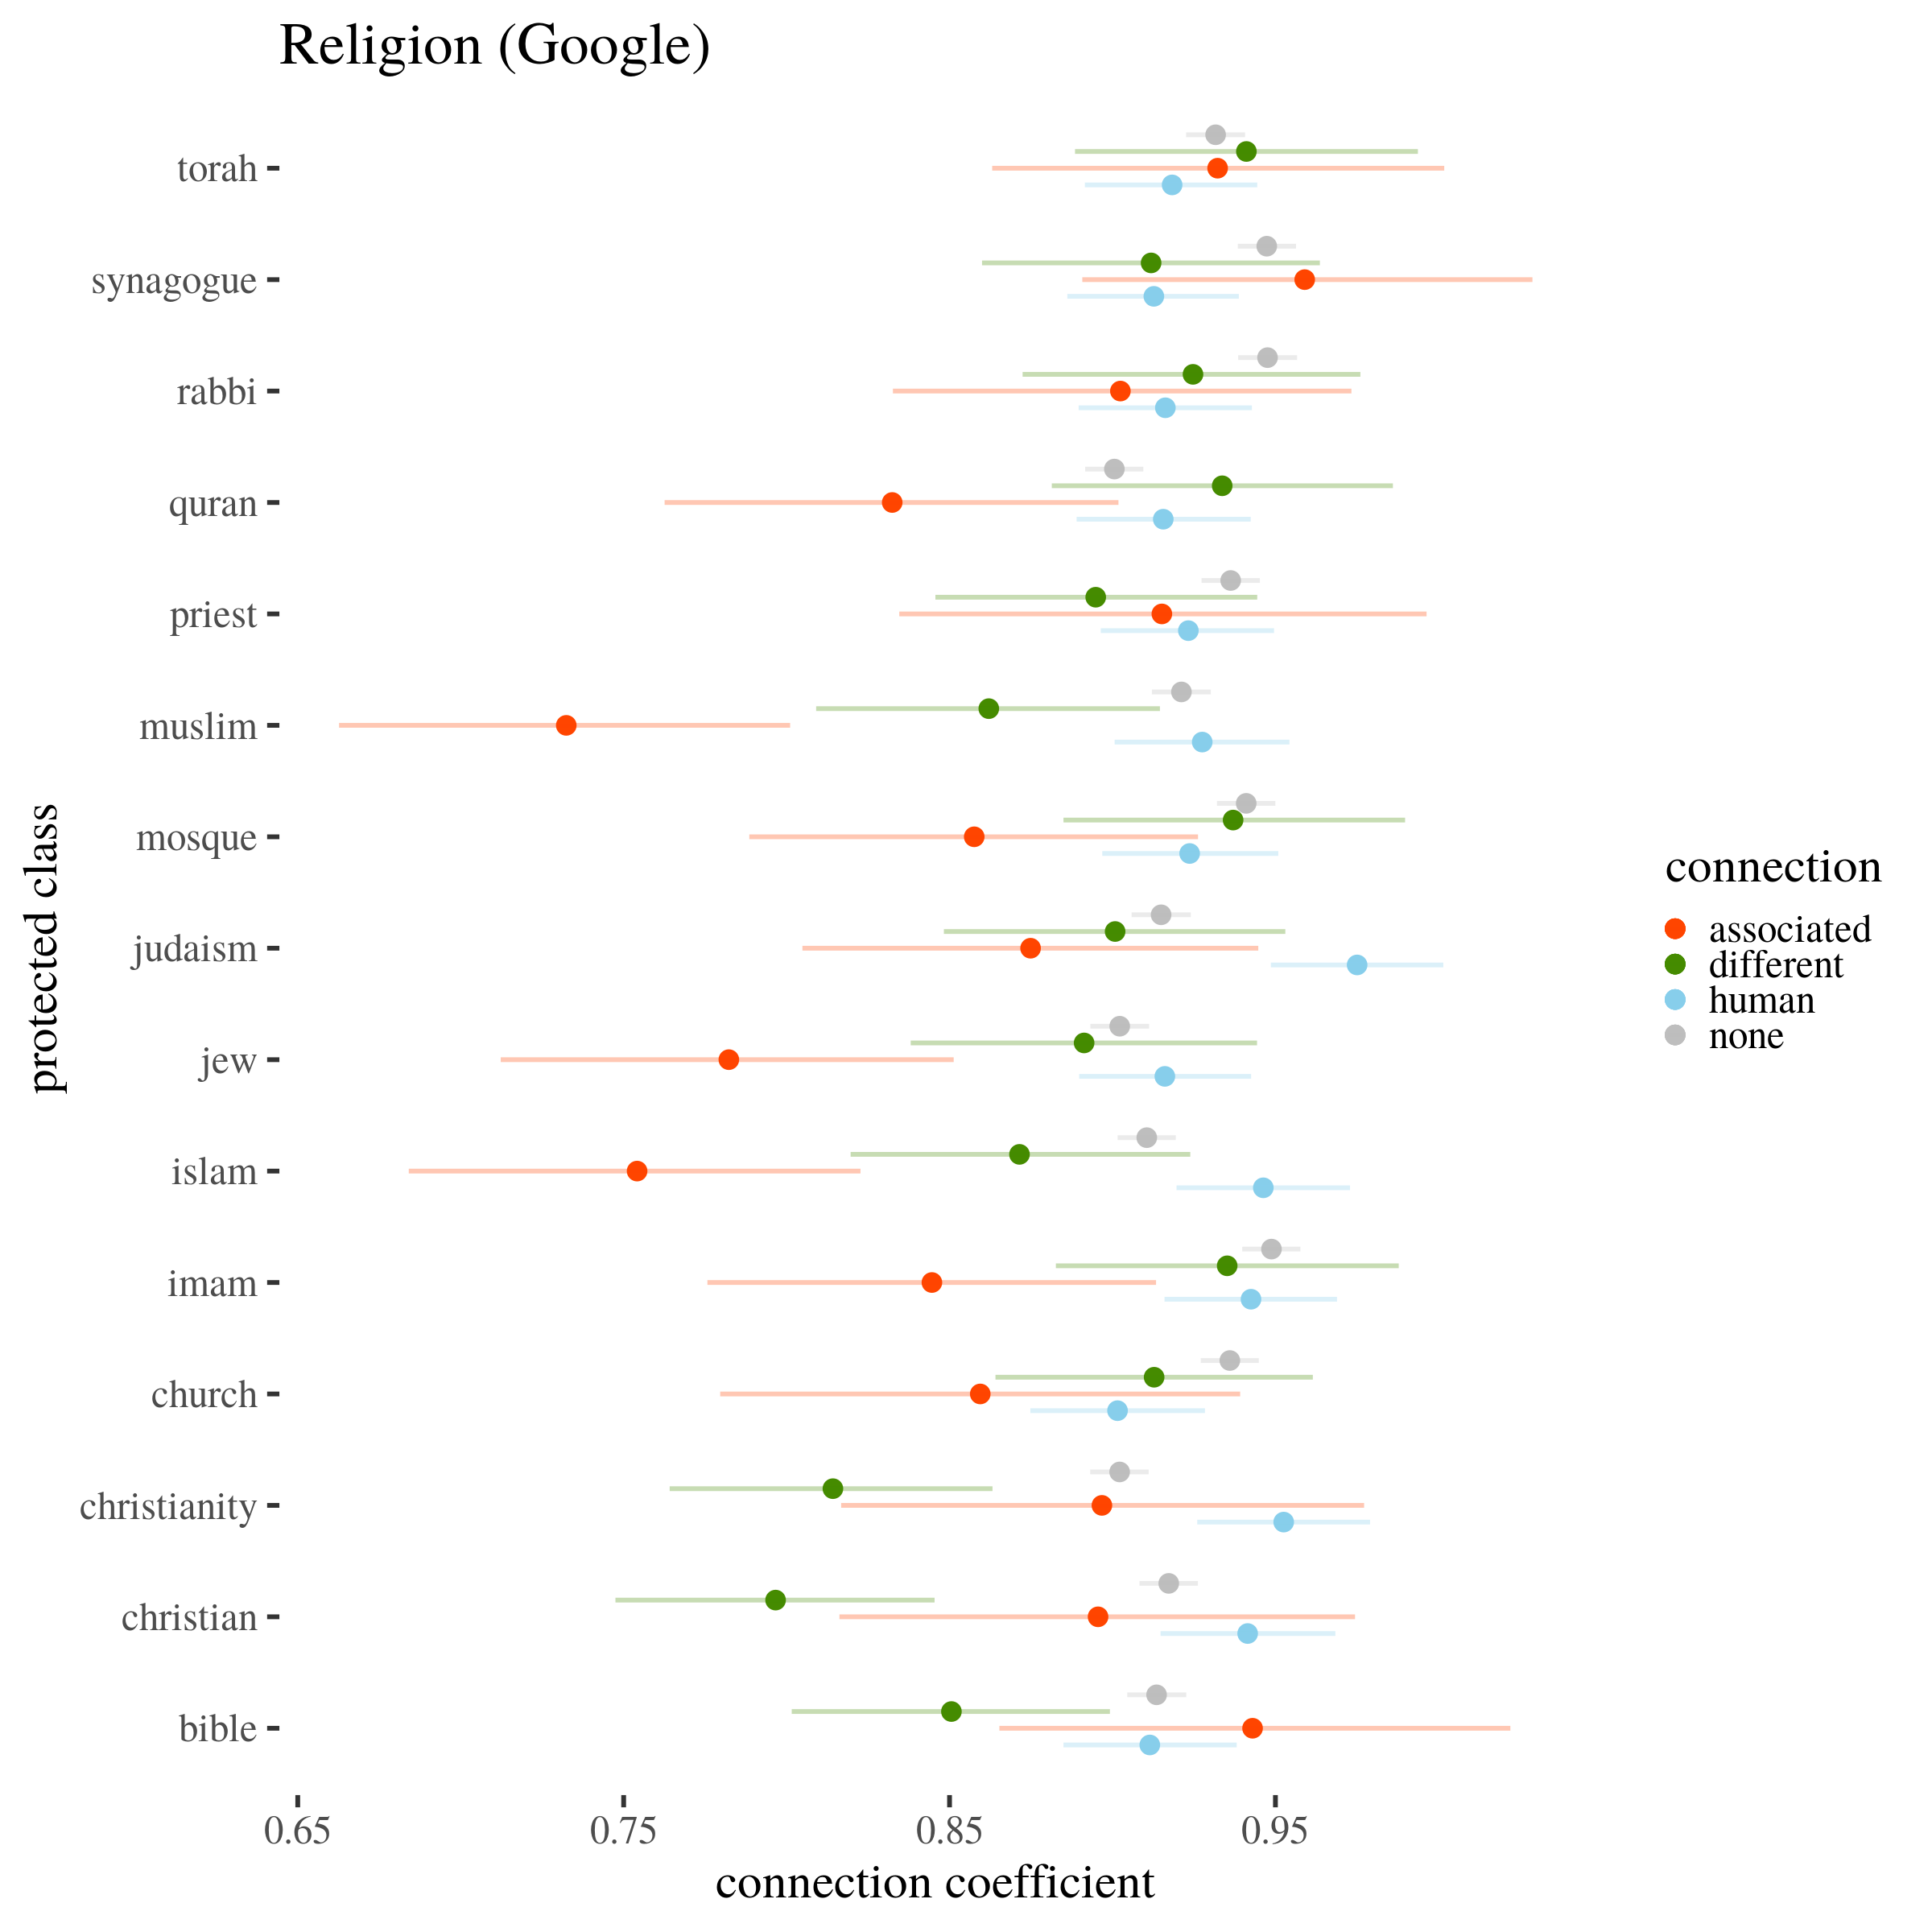
\includegraphics[width=14cm]{../images/visReligionGoogle.png}

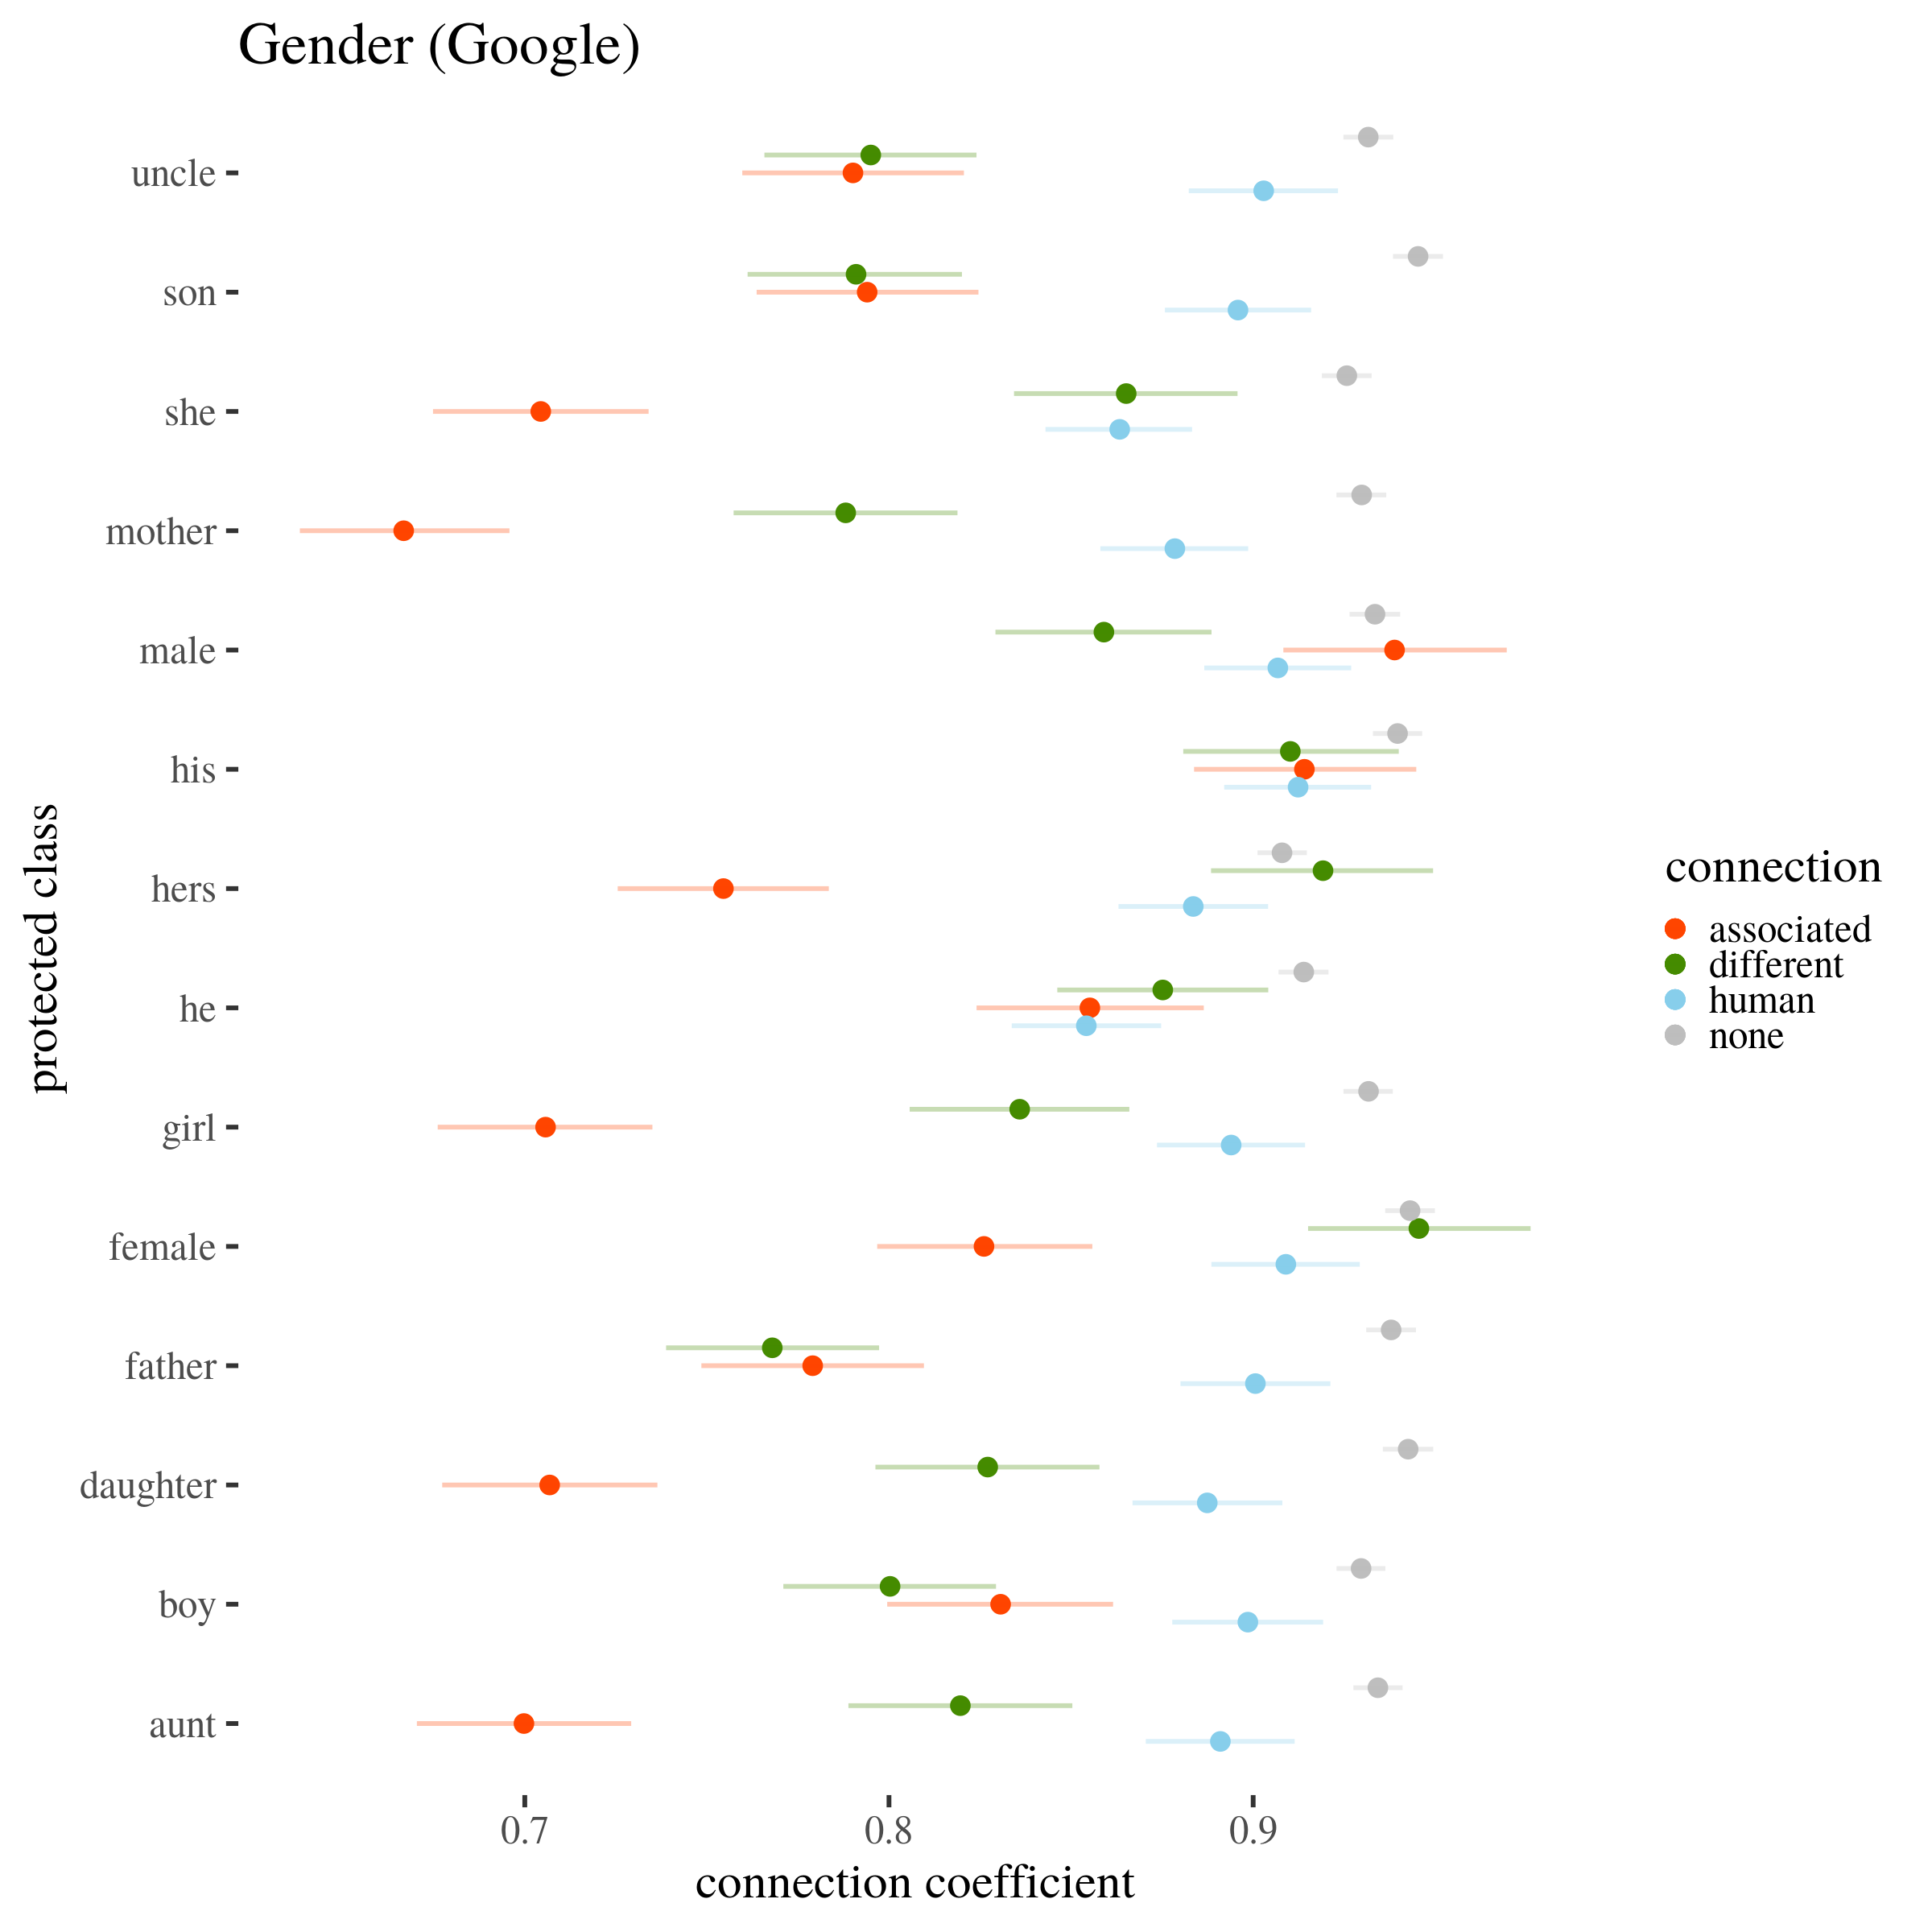
\includegraphics[width=14cm]{../images/visGenderGoogle.png}

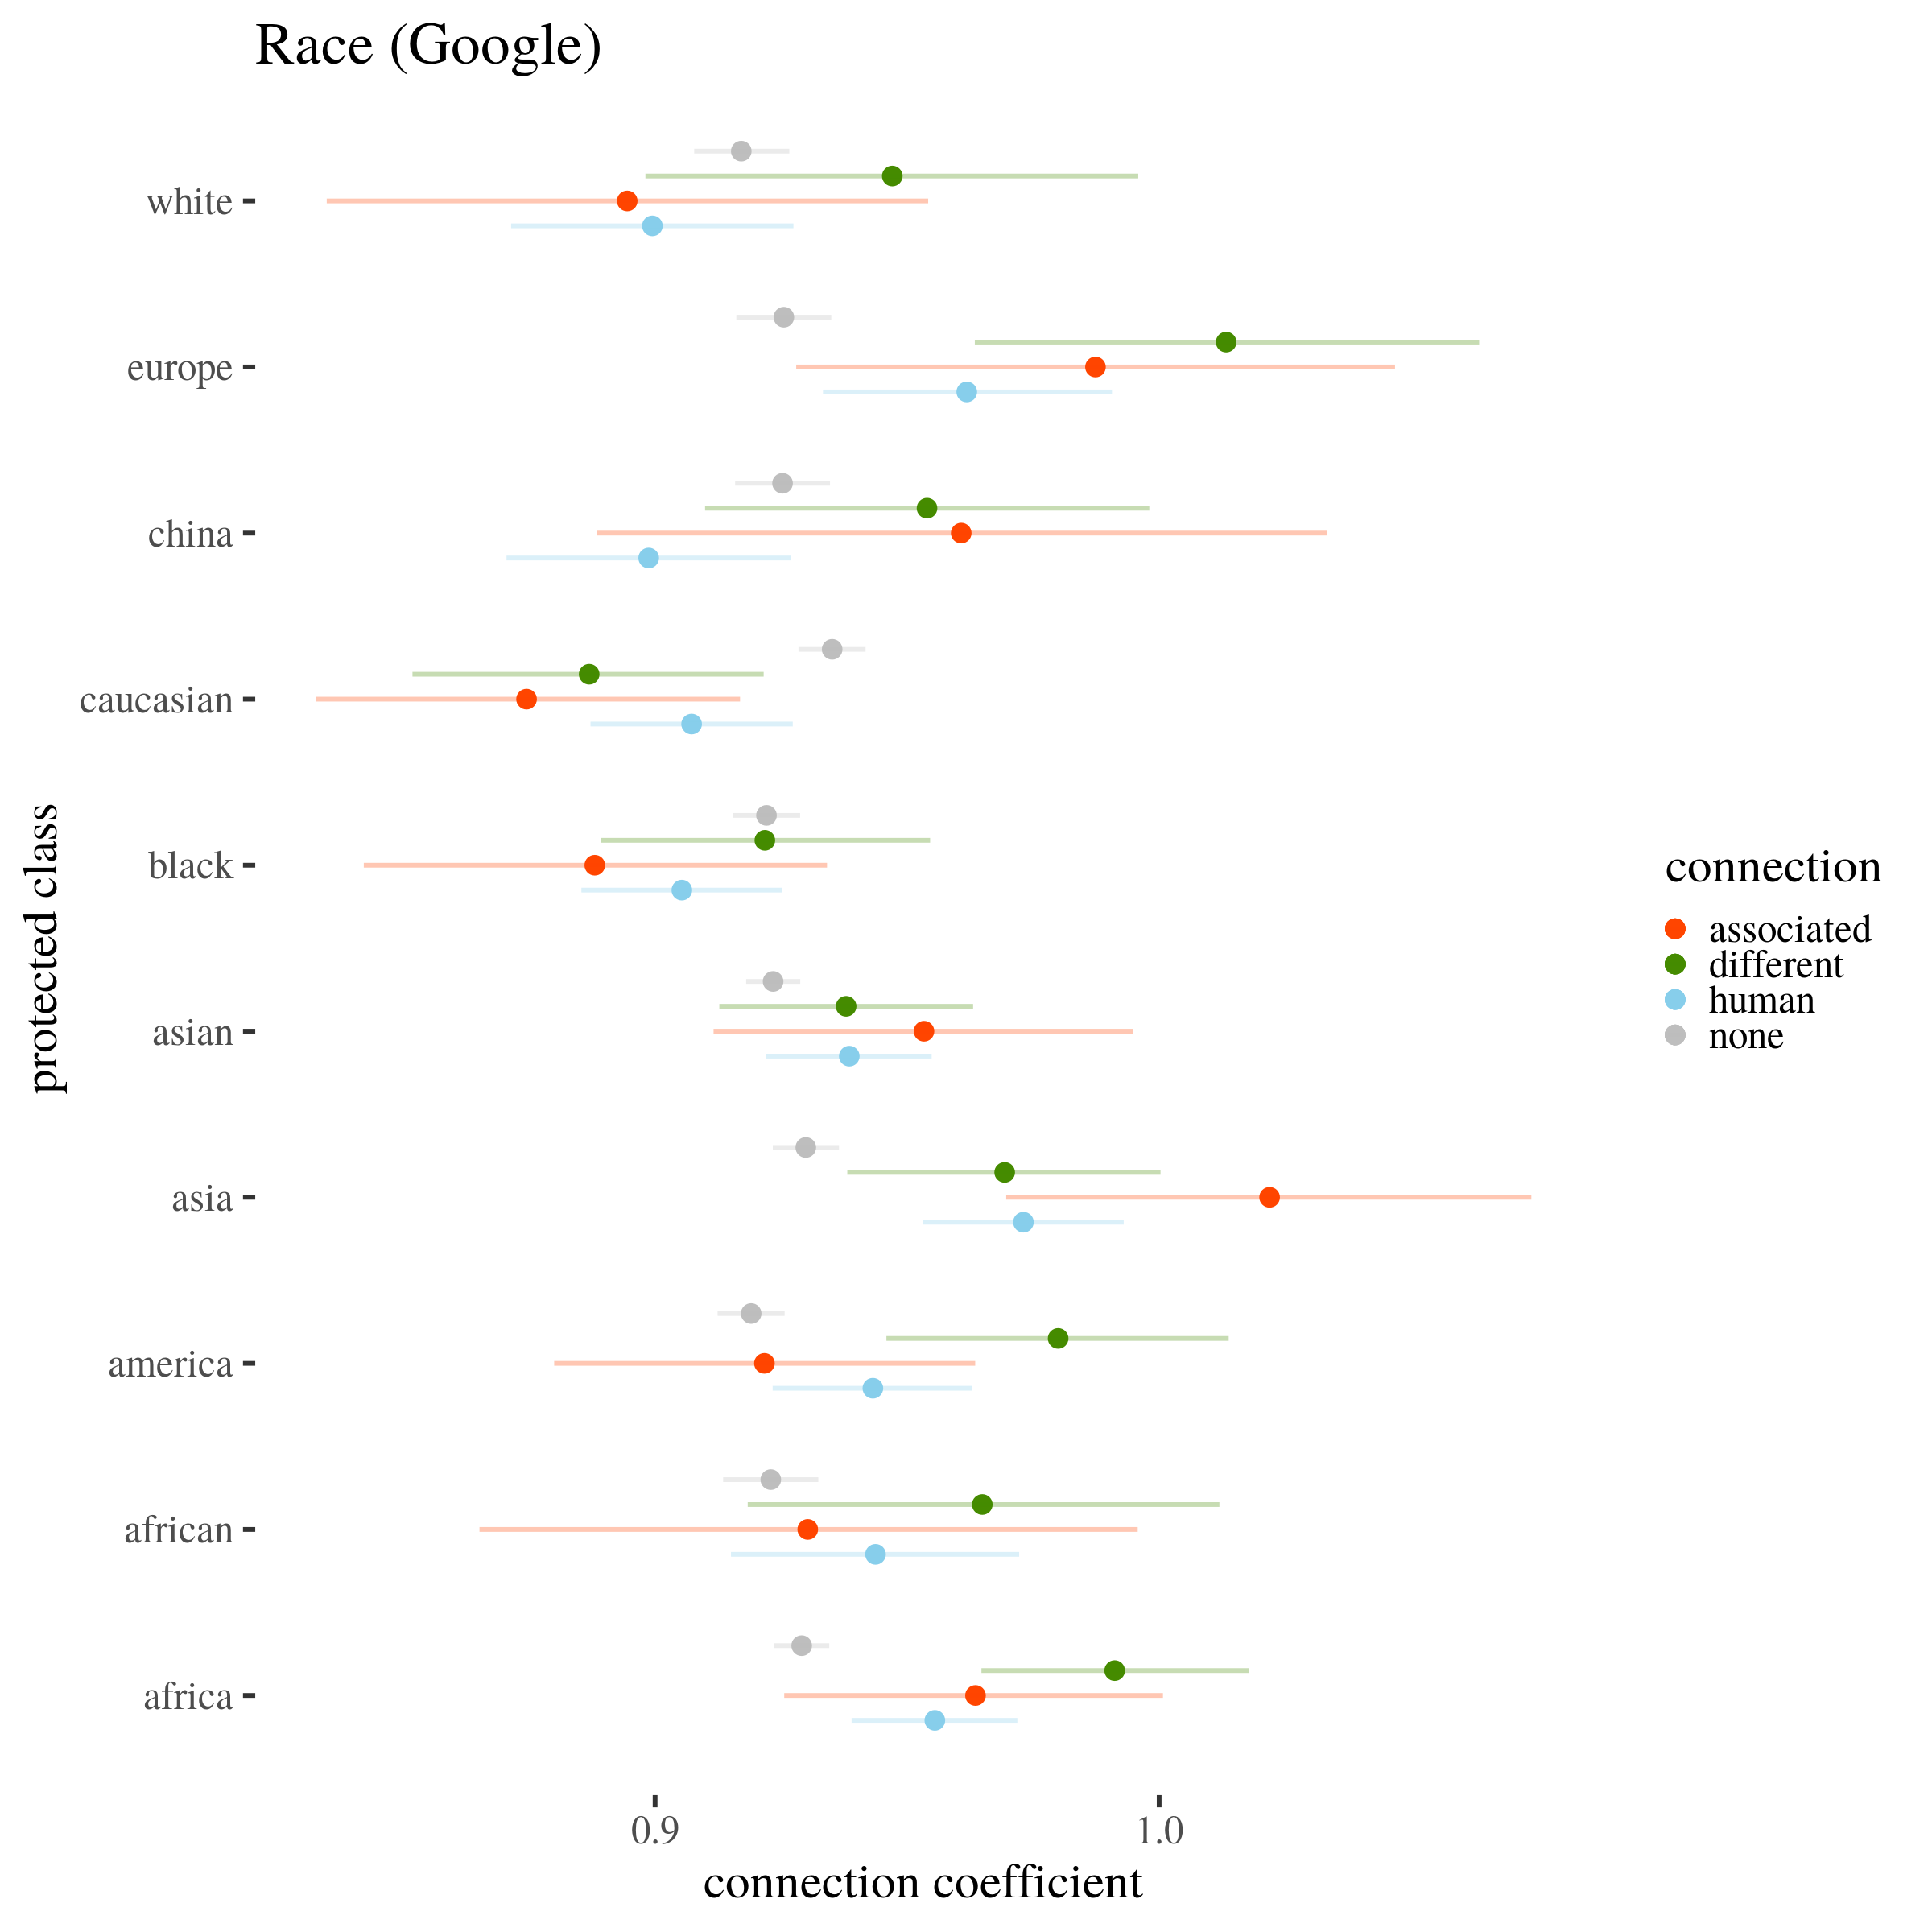
\includegraphics[width=14cm]{../images/visRaceGoogle.png}

We leave a discussion of these results for later, for now let us also inspect the impact of debiasing.

\hypertarget{the-role-of-debiasing}{%
\chapter{The role of debiasing}\label{the-role-of-debiasing}}

We also applied to the word embeddings hard debiasing method found in \protect\hyperlink{ref-Manzini2019blackToCriminal}{Manzini, Lim, Tsvetkov, \& Black} (\protect\hyperlink{ref-Manzini2019blackToCriminal}{2019}). As it was mentioned before, debiasing consists of two components: identifying the bias subspace and then removing this vector subspace from the chosen embeddings. The aim is to increase the cosine distance between protected words and the set of attributes.
After debiasing the Reddit word embeddings we calculated the cosine distance again to see if there are any significant changes in terms of the similarity between protected words and the attributes.

\hypertarget{dataset-level-coefficients-after-debiasing}{%
\section{Dataset-level coefficients after debiasing}\label{dataset-level-coefficients-after-debiasing}}

First, let's look at coefficient estimated for the whole datasets, as compared to their estimation prior to debiasing. One may observe very slight changes in the estimated coefficients. It seems that in religion dataset the changes are the most significant as the mean moves towards zero which stands for no similarity between words.

\begin{center}
\begin{figure}[!htb]\centering
   \begin{minipage}{0.55\textwidth}
  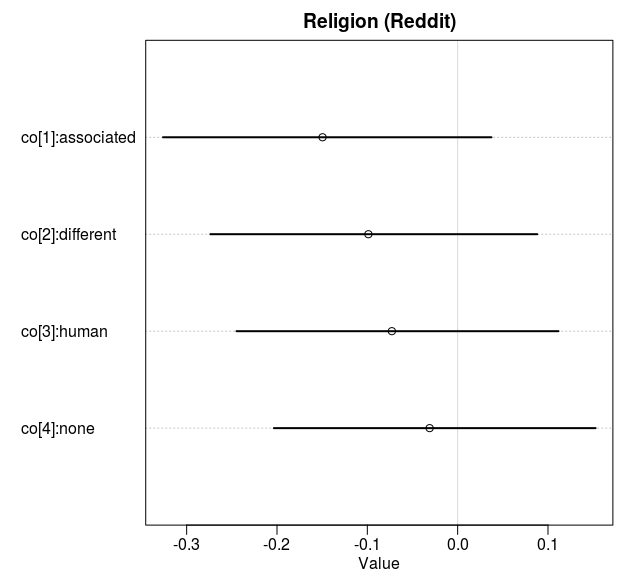
\includegraphics[width=7cm]{../images/religionCoeffs.jpeg}
   \end{minipage}
   \begin {minipage}{0.43\textwidth}
    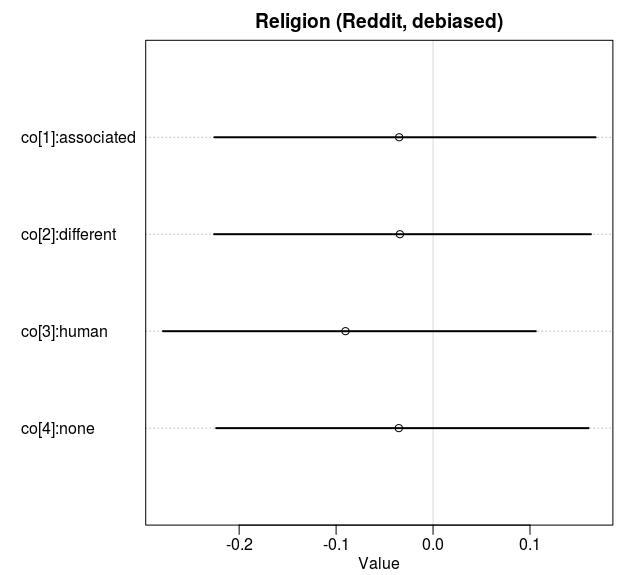
\includegraphics[width=7cm]{../images/debiasedReligionRedditCoeffs.jpeg}
   \end{minipage}
   
   
  \begin{minipage}{0.55\textwidth}
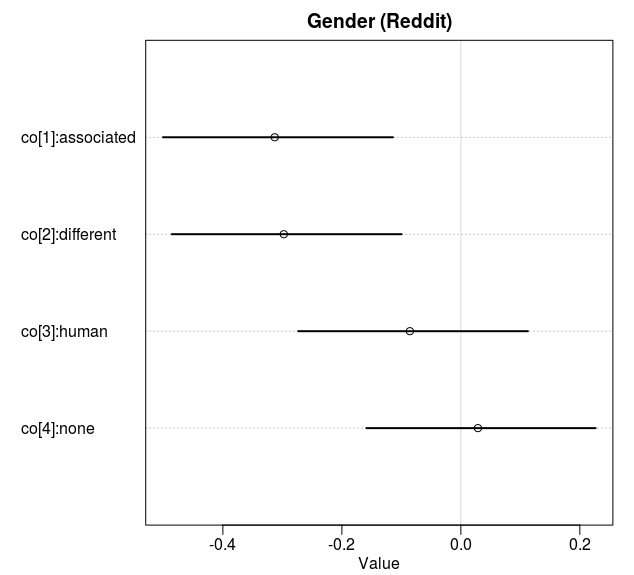
\includegraphics[width=7cm]{../images/genderCoeffs.jpeg}
\end{minipage}
   \begin {minipage}{0.43\textwidth}
    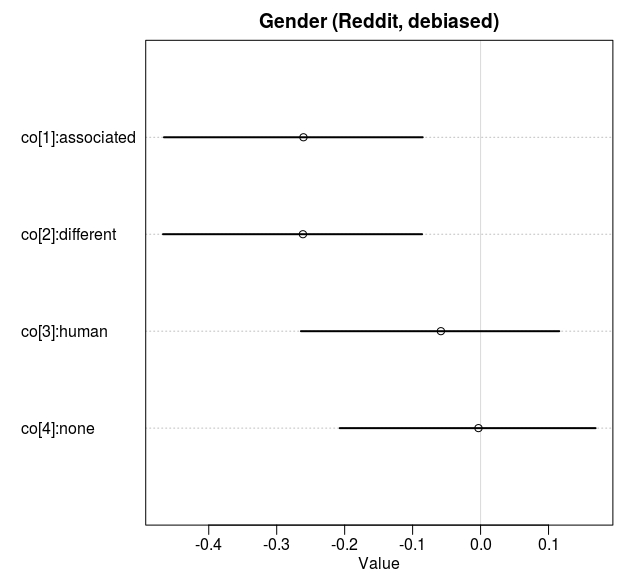
\includegraphics[width=7cm]{../images/debiasedGenderRedditCoeffs.jpeg}
   \end{minipage}
   
   
   
   
  \begin{minipage}{0.55\textwidth}
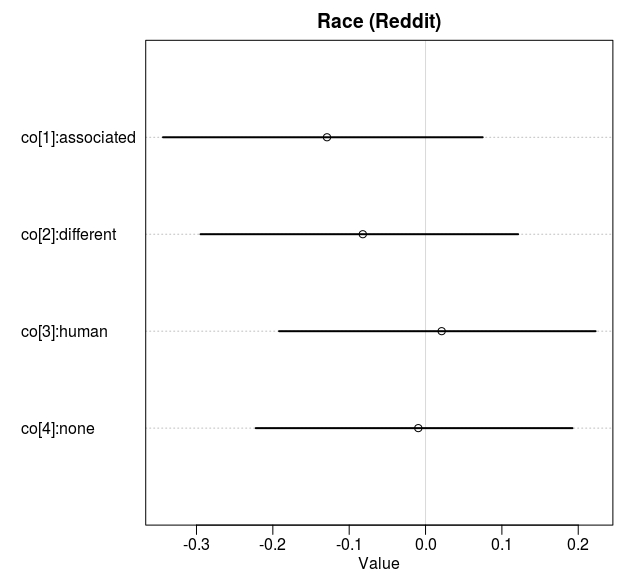
\includegraphics[width=7cm]{../images/raceCoeffs.jpeg}
\end{minipage}
   \begin {minipage}{0.43\textwidth}
    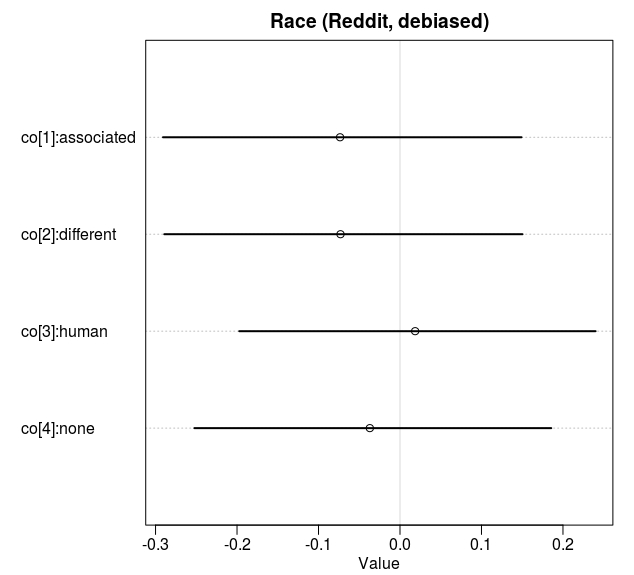
\includegraphics[width=7cm]{../images/debiasedRaceRedditCoeffs.jpeg}
   \end{minipage}
\end{figure}

\end{center}

\hypertarget{protected-classes-after-debiasing}{%
\section{Protected classes after debiasing}\label{protected-classes-after-debiasing}}

Now, perhaps, the effects of debiasing will be better appreciated if we look at the level of protected words. After all, the hope is, the situation of extremely ill-positioned protected words have improved?

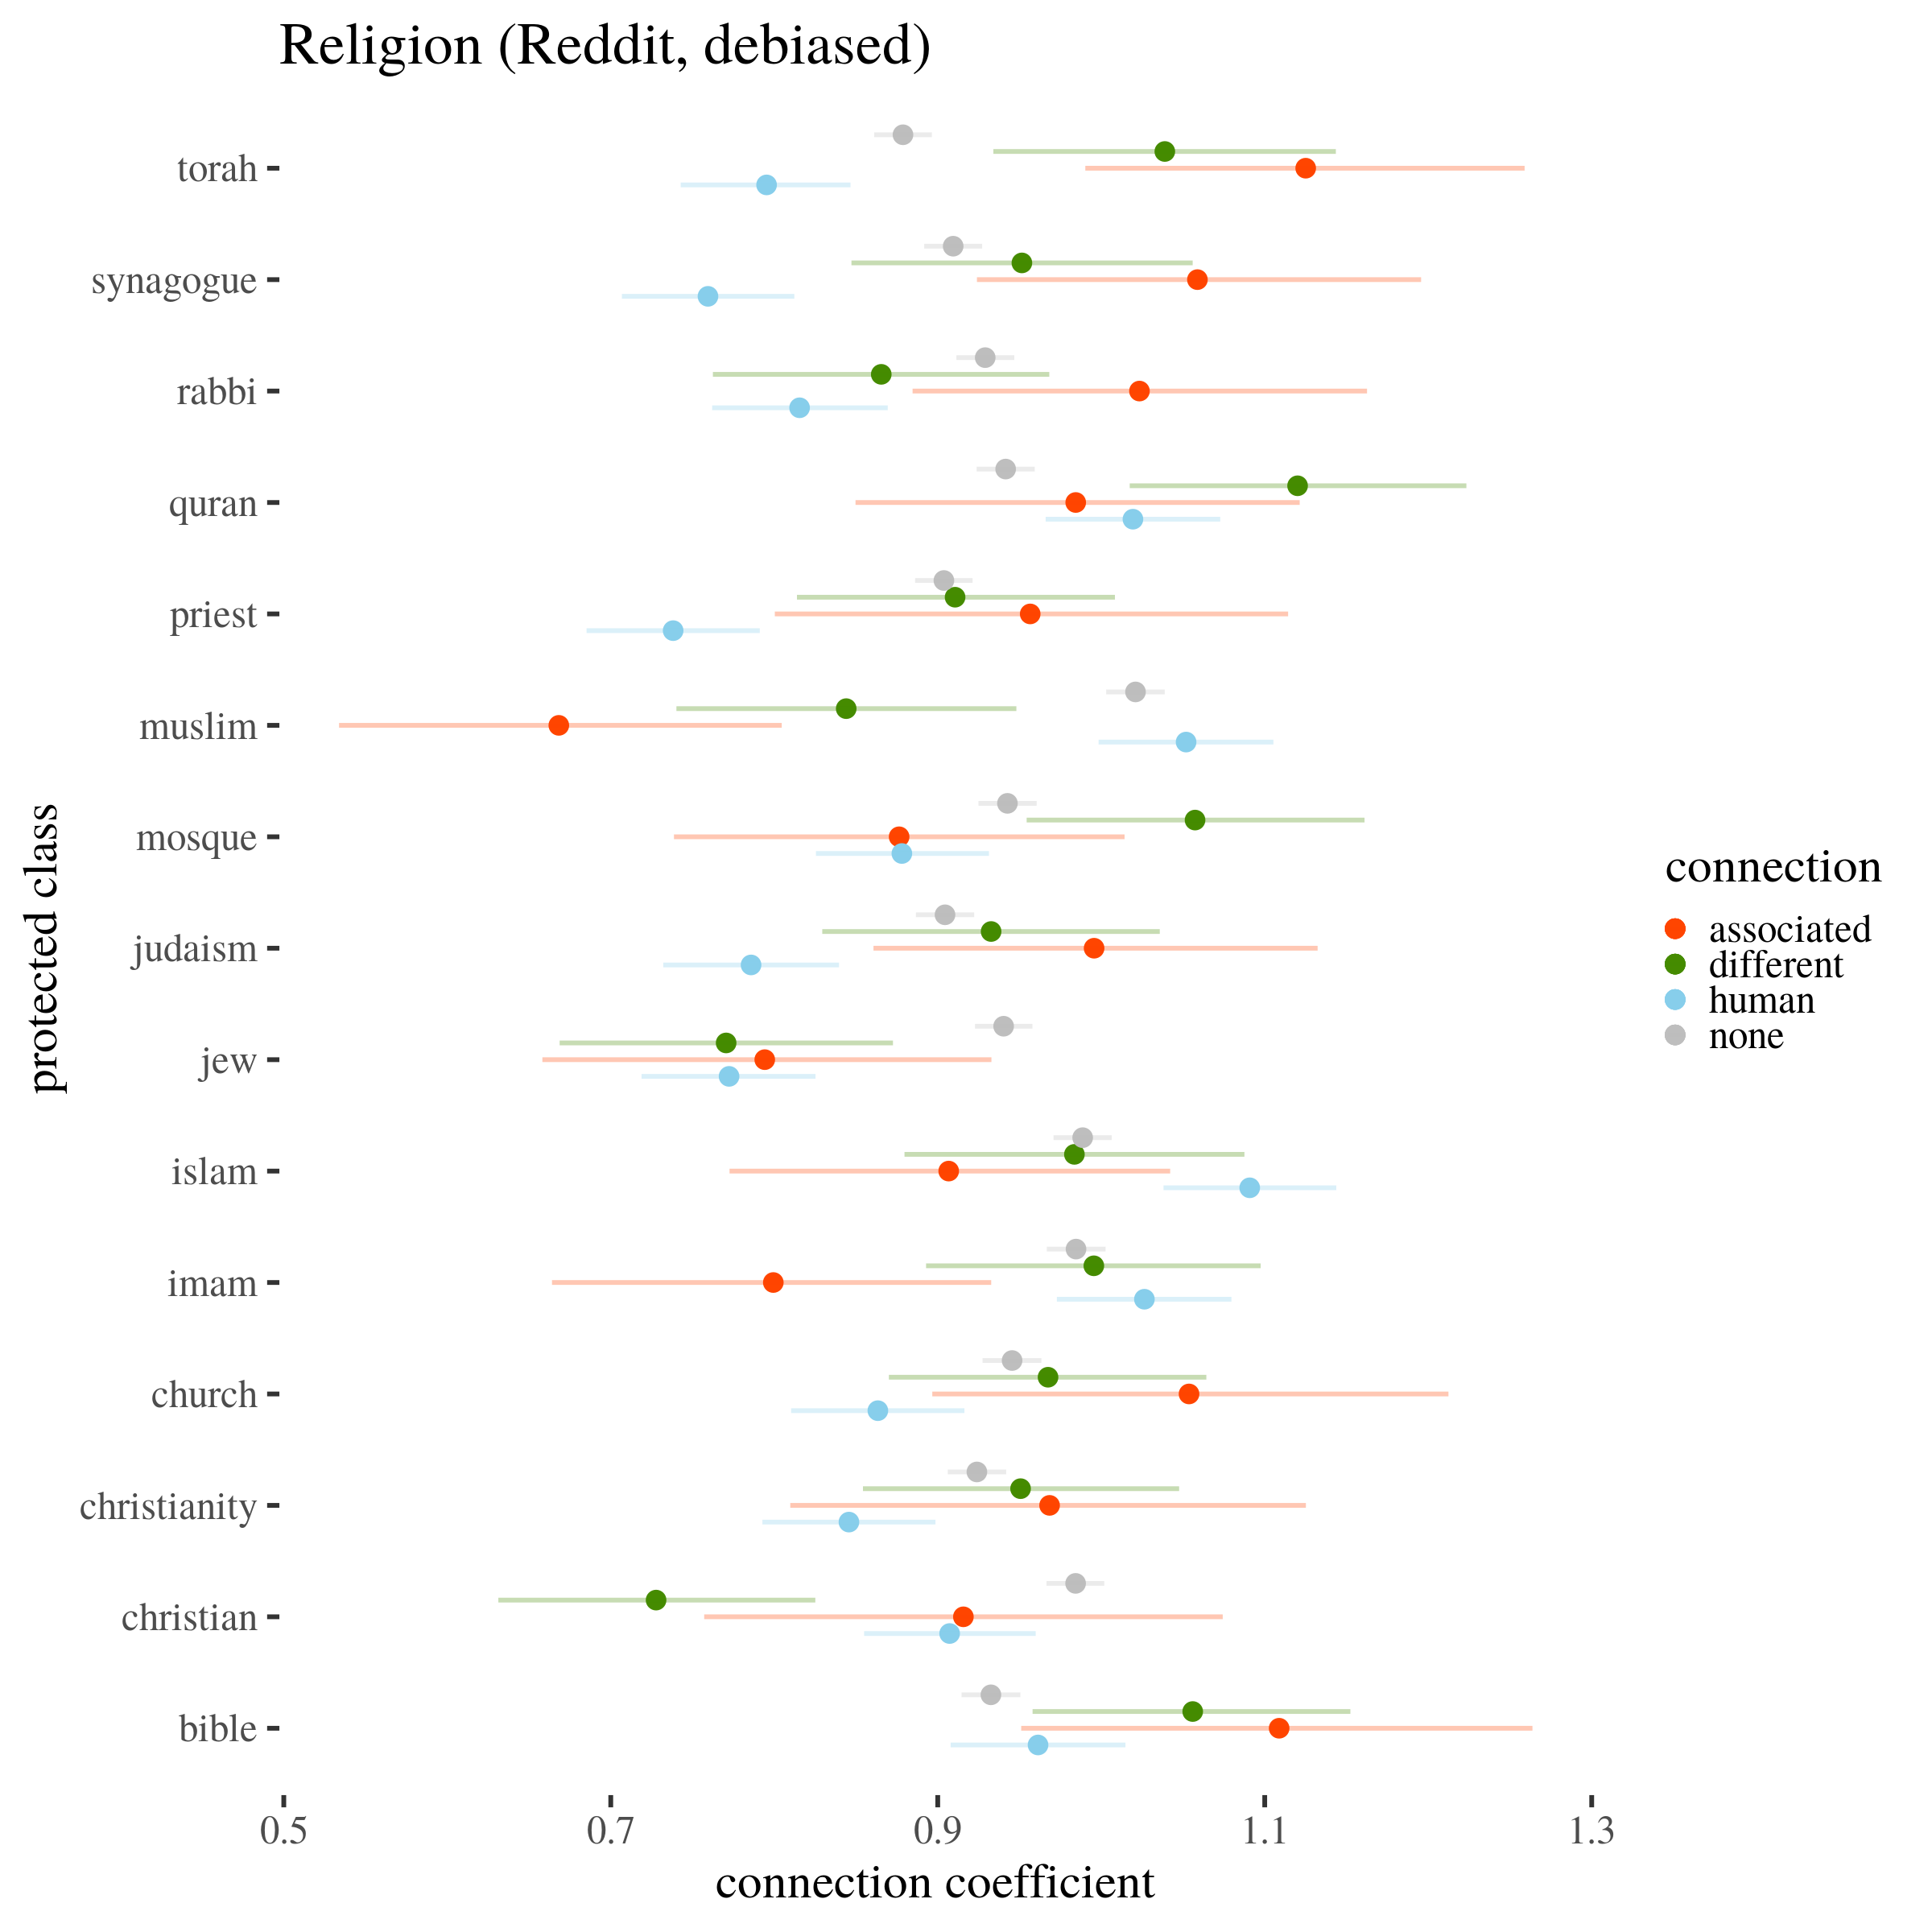
\includegraphics[width=14cm]{../images/visDebReligionReddit.png}

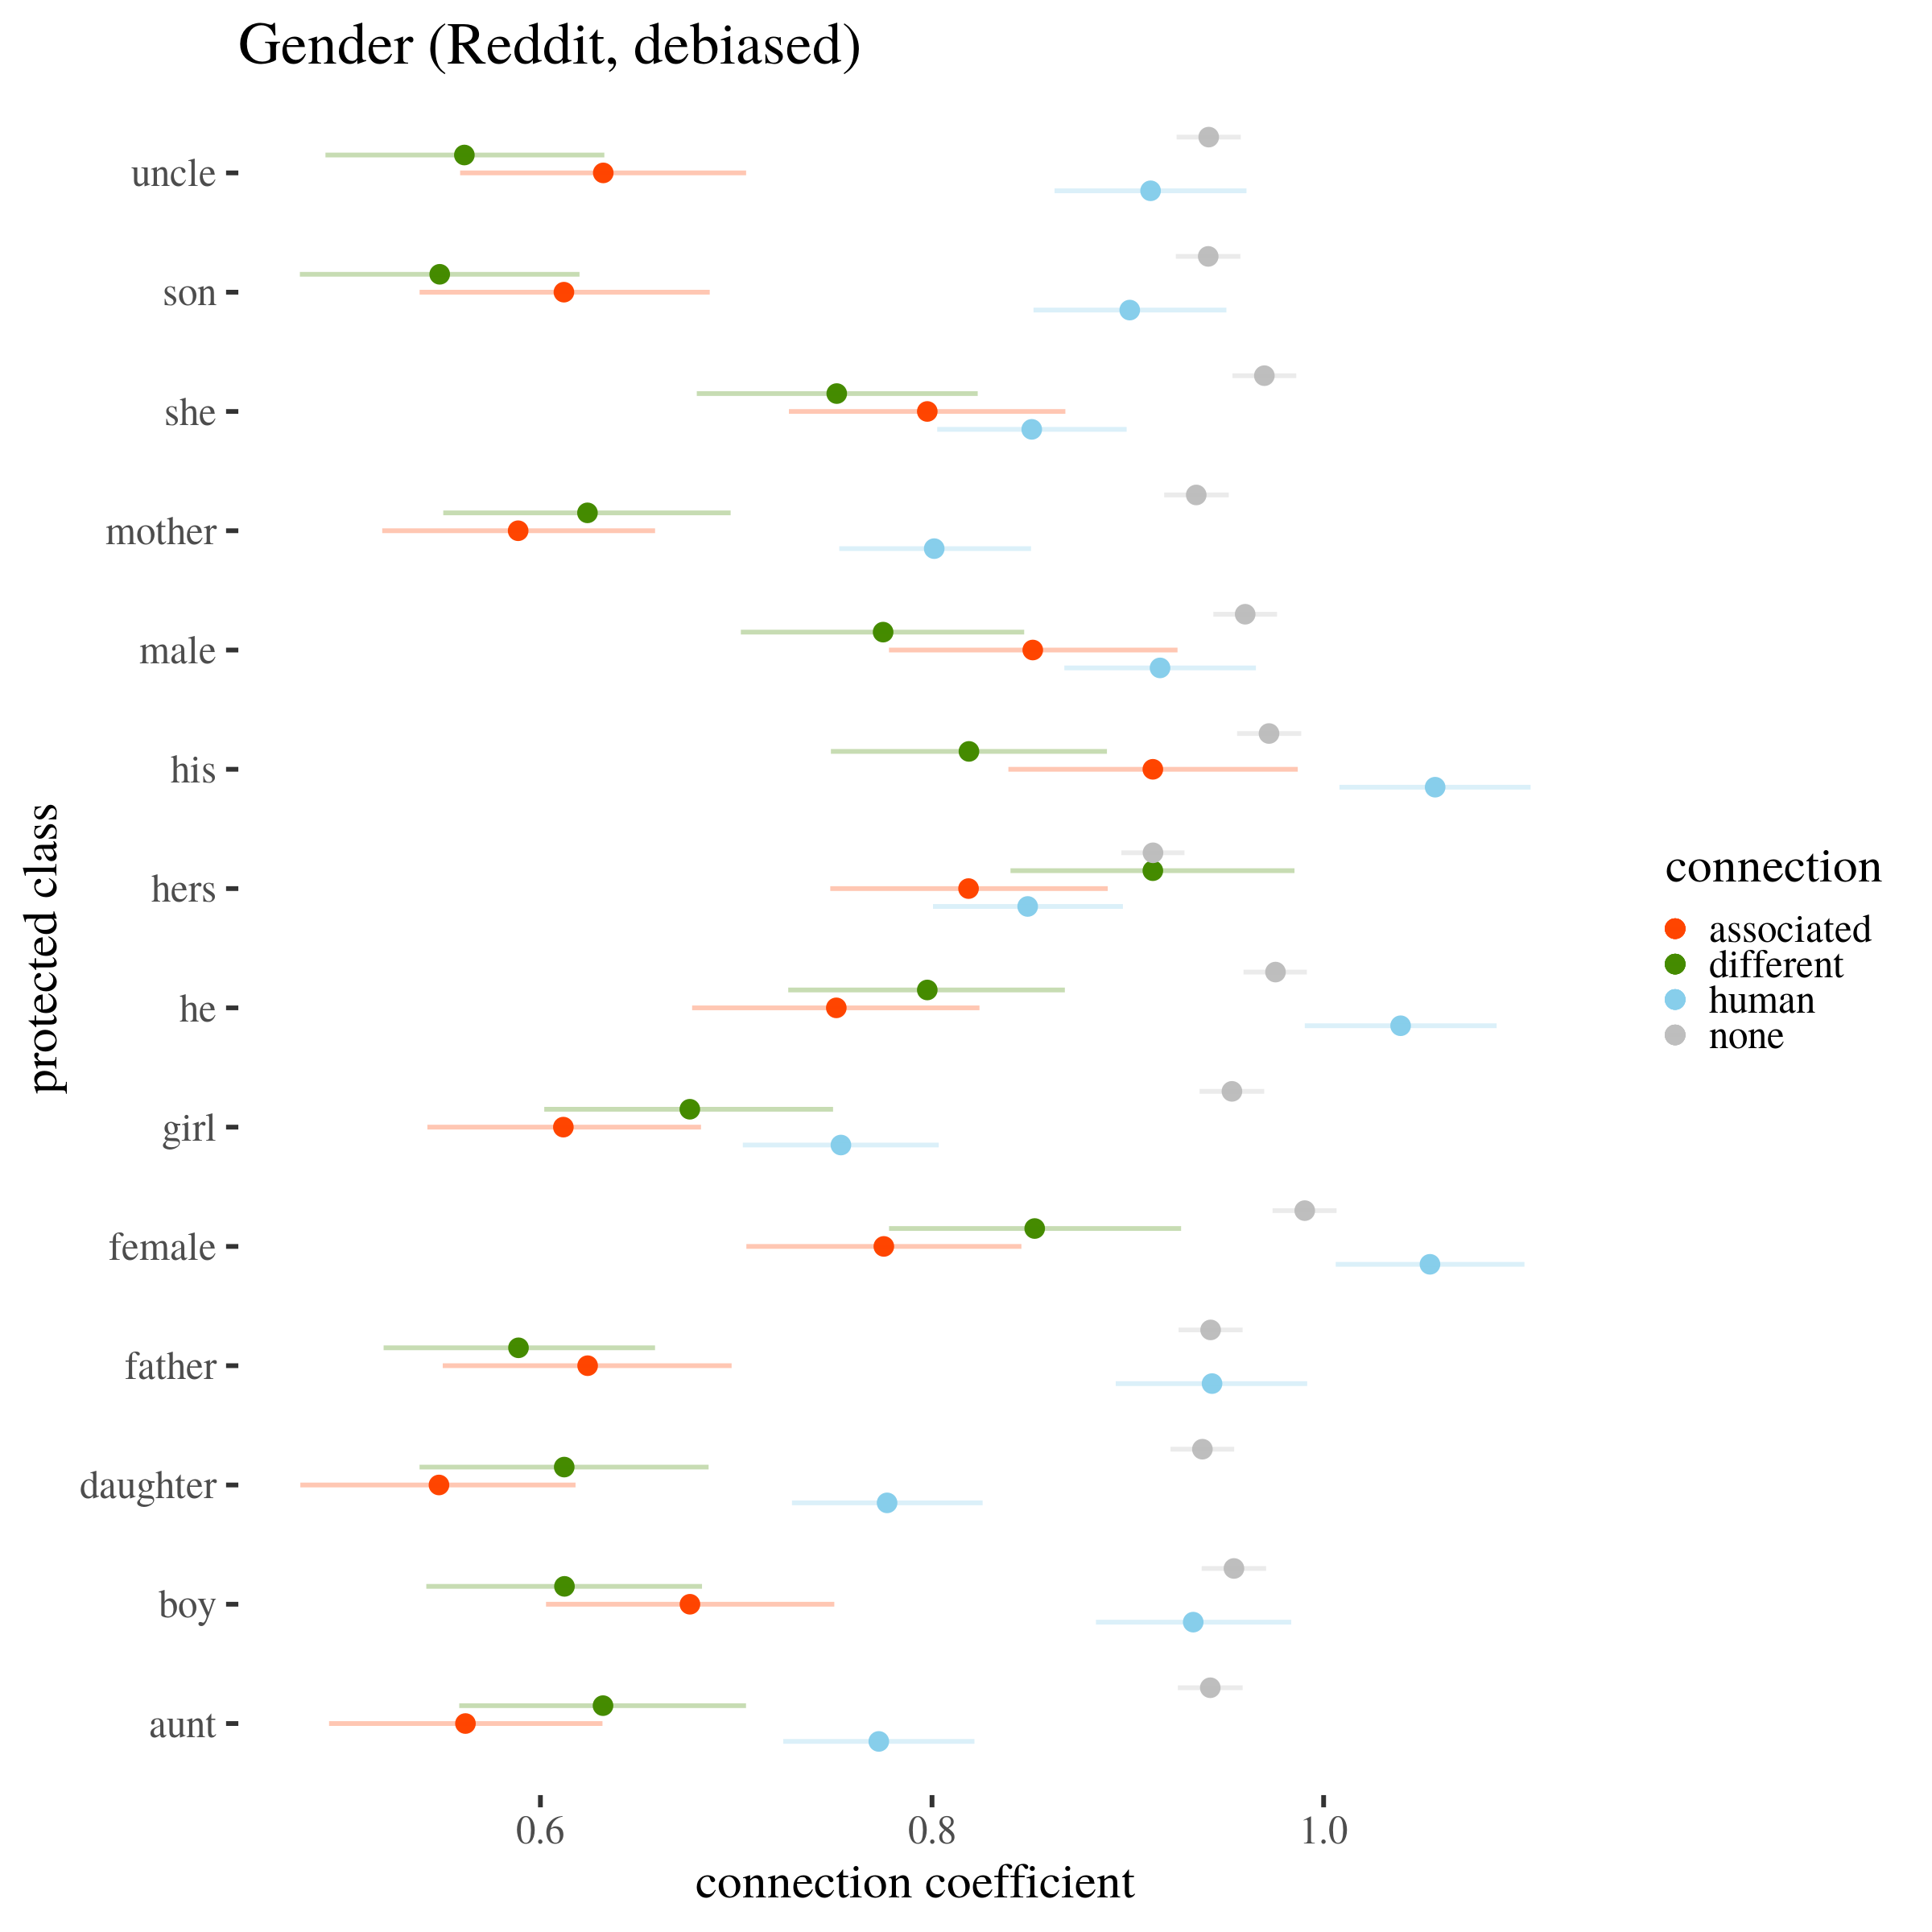
\includegraphics[width=14cm]{../images/visDebGenderReddit.png}

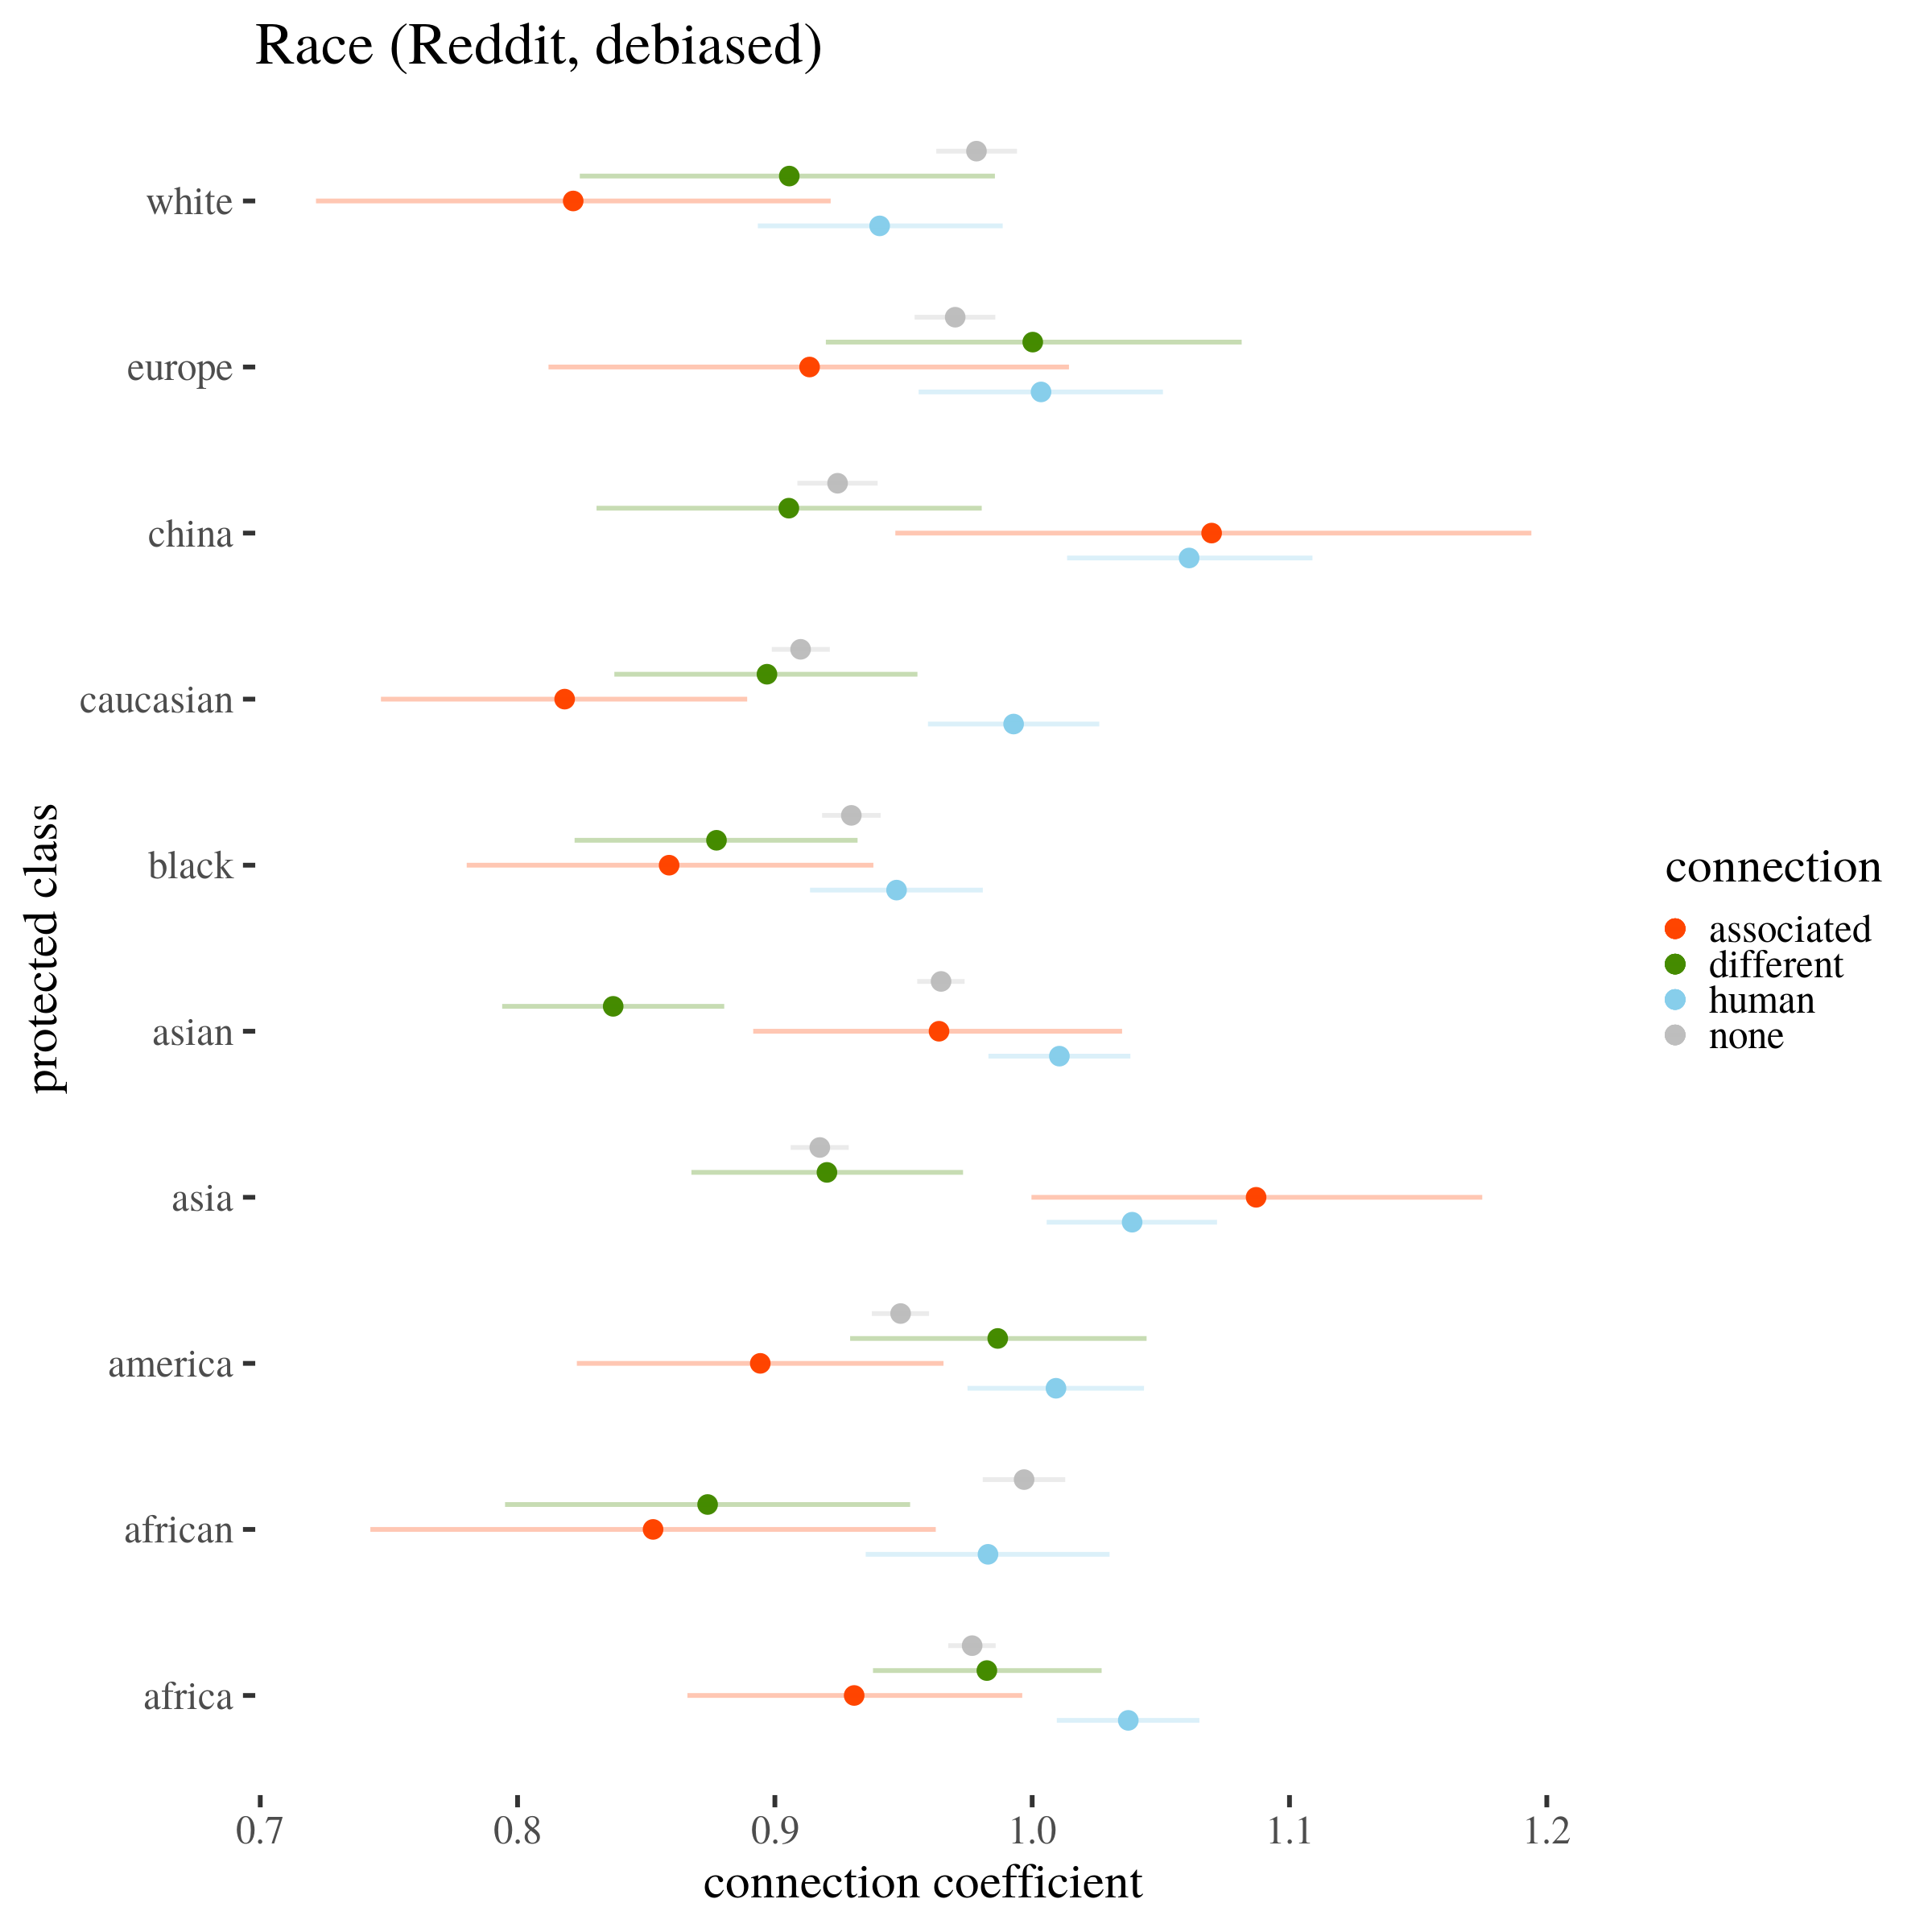
\includegraphics[width=14cm]{../images/visDebRaceReddit.png}

One may notice that in a religion data set most of the distances for \texttt{associated} words slightly increased. Some of the distances from \texttt{different} class are still smaller than for the \texttt{associated} class. The distances for all classes seem in most cases to cluster together even after debiasing. The reason may be that uncertainty is quite high in \texttt{associated} and \texttt{different} class because the number of samples is so small. Additionally in some cases distances from \texttt{human} class are smaller than for the \texttt{assosiated} class which also makes it less clear how to interpret the results, if the distances are really able to catch the bias presence.

It is worth paying attention to the gender debiased dataset. The change is really minor, still with zero out of the HPDI range. The \texttt{different} attributes still have high similarity value. It seems that the distances for gender protected words are still clustered together which suggests that this method is unable to catch the complex bias presence. One could conclude that co-occurrence of certain terms does not always mean direct connection in terms of terms associations. The fact that some of stereotypically associated with female attributes still have high similarity with male protected words suggest that other techniques should be applied to detect and remove the bias.

At the same time, there is a small improvement in race dataset. In some cases the distances just cluster together. In general distances for \texttt{assosiated} class are still higher than those for the rest of classes. One may assume that there reason for so small change is that either the metric does not indicate properly biases or that the issue is more complex and subtracting subspaces is not enough.

\hypertarget{discussion-and-summary}{%
\chapter{Discussion and summary}\label{discussion-and-summary}}

Placeholder

\hypertarget{appendix}{%
\chapter*{Appendix}\label{appendix}}
\addcontentsline{toc}{chapter}{Appendix}

Placeholder

\hypertarget{original-wordlist-from-manzini2019blacktocriminal}{%
\section*{\texorpdfstring{Original wordlist from (\protect\hyperlink{ref-Manzini2019blackToCriminal}{Manzini, Lim, Tsvetkov, \& Black, 2019})}{Original wordlist from (Manzini, Lim, Tsvetkov, \& Black, 2019)}}\label{original-wordlist-from-manzini2019blacktocriminal}}
\addcontentsline{toc}{section}{Original wordlist from (\protect\hyperlink{ref-Manzini2019blackToCriminal}{Manzini, Lim, Tsvetkov, \& Black, 2019})}

\hypertarget{religion}{%
\subsection*{Religion}\label{religion}}
\addcontentsline{toc}{subsection}{Religion}

\hypertarget{gender}{%
\subsection*{Gender}\label{gender}}
\addcontentsline{toc}{subsection}{Gender}

\hypertarget{race}{%
\subsection*{Race}\label{race}}
\addcontentsline{toc}{subsection}{Race}

\hypertarget{our-control-groups}{%
\section*{Our control groups}\label{our-control-groups}}
\addcontentsline{toc}{section}{Our control groups}

\hypertarget{human-neutral-attributes}{%
\section*{Human neutral attributes}\label{human-neutral-attributes}}
\addcontentsline{toc}{section}{Human neutral attributes}

\hypertarget{non-human-neutral-attributes}{%
\section*{Non-human neutral attributes}\label{non-human-neutral-attributes}}
\addcontentsline{toc}{section}{Non-human neutral attributes}

\hypertarget{refs}{}
\begin{CSLReferences}{1}{0}
\leavevmode\hypertarget{ref-Bolukbasi2016Man}{}%
Bolukbasi, T., Chang, K.-W., Zou, J. Y., Saligrama, V., \& Kalai, A. (2016). Man is to computer programmer as woman is to homemaker? Debiasing word embeddings. \emph{CoRR}, \emph{abs/1607.06520}. Retrieved from \url{http://arxiv.org/abs/1607.06520}

\leavevmode\hypertarget{ref-Manzini2019blackToCriminal}{}%
Manzini, T., Lim, Y. C., Tsvetkov, Y., \& Black, A. W. (2019). Black is to criminal as caucasian is to police: Detecting and removing multiclass bias in word embeddings. Retrieved from \url{http://arxiv.org/abs/1904.04047}

\end{CSLReferences}

\end{document}
